\documentclass[]{interact}

\usepackage[utf8]{inputenc}
\usepackage{algorithm}
\usepackage{algorithmic}
\usepackage{geometry}
\geometry{margin=1in}

\usepackage{amsfonts} 
\usepackage{amssymb}
\usepackage{enumitem}
\usepackage{listings}
\usepackage{xcolor}
\lstset{
    basicstyle=\ttfamily\footnotesize,
    breaklines=true,
    frame=single,
    backgroundcolor=\color{gray!10}
}

\usepackage[utf8]{inputenc}
\usepackage[T1]{fontenc}
\usepackage{amsmath,amsfonts,amssymb}
\usepackage{graphicx}
\usepackage{booktabs}
\usepackage{array}
\usepackage{longtable}
\usepackage{multirow}
\usepackage{subcaption}
\usepackage{hyperref}

% Use Latin Modern fonts
\usepackage{lmodern}
\usepackage{float}
\usepackage{graphicx}
% To incorporate .eps illustrations using PDFLaTeX
\usepackage{epstopdf}
% Citation support using natbib.sty
\usepackage[numbers,sort&compress]{natbib}
% Citation support using natbib.sty
\bibpunct[, ]{[}{]}{,}{n}{,}{,}
% Bibliography support using natbib.sty
\renewcommand\bibfont{\fontsize{10}{12}\selectfont}
% @ becomes a letter
\makeatletter
% Suppress spaces between citations using natbib.sty
\def\NAT@def@citea{\def\@citea{\NAT@separator}}
% @ becomes a symbol again
\makeatother
% Theorem-like structures provided by amsthm.sty
\theoremstyle{plain}
\newtheorem{theorem}{Theorem}[section]
\newtheorem{lemma}[theorem]{Lemma}
\newtheorem{corollary}[theorem]{Corollary}
\newtheorem{proposition}[theorem]{Proposition}
% 
\theoremstyle{definition}
\newtheorem{definition}[theorem]{Definition}
\newtheorem{example}[theorem]{Example}
%
\theoremstyle{remark}
\newtheorem{remark}{Remark}
\newtheorem{notation}{Notation}







\begin{document}


\articletype{RESEARCH ARTICLE}

\title{Optimistic Static Data Partitioning for Cost-Aware Parallel Sorting in Heterogeneous Distributed Systems}

\author{
\name{Joeniño Cainday and Junar Landicho}
% TODO: thanks is on the template
% \thanks{CONTACT Joeniño Cainday. Email: caindayjoeninyo@gmail.com}
\affil{Department of Computer Science, University of Science and Technology of Southern Philippines, Cagayan De Oro City, Philippines}
}

\maketitle

\begin{abstract}
This research addresses the challenge of efficient static data partitioning for parallel sorting in heterogeneous distributed systems, aiming to minimize both execution time (makespan) and monetary cost. Current methods often struggle with load balancing and resource utilization, particularly in cost-sensitive cloud environments. We introduce Heterogeneous Parallel Sorting by Linear Programming (H-PSLP), an approach that employs a linear programming (LP) model to determine optimal data allocation across nodes with varying performance, memory capacities, and costs. H-PSLP replaces the heuristic, sampling-based partitioning phase of traditional algorithms like Heterogeneous Parallel Sorting by Regular Sampling (H-PSRS), which serves as our primary performance benchmark.

Simulations were conducted using synthetic datasets (uniform and Gaussian distributions) and heterogeneous cluster configurations (4 and 8 nodes). The results demonstrate H-PSLP's superiority over H-PSRS. Across all experiments, H-PSLP achieved an average makespan reduction of 33.3\% and an average total cost reduction of 60.7\% compared to H-PSRS. Critically, H-PSLP consistently adhered to node memory constraints, preventing the memory overflows that plagued H-PSRS in all tested scenarios. The LP optimization overhead was minimal, and H-PSLP proved robust to different data distributions and scaled effectively. These findings highlight H-PSLP as a more reliable, efficient, and economically viable solution for parallel sorting in heterogeneous environments. Future work will focus on distributed merge strategies and refining the LP model.
\end{abstract}

\begin{keywords}
Data Partitioning, Parallel Sorting, Heterogeneous Distributed Systems, Cost Optimization, Makespan Minimization, Linear Programming, Resource Allocation, Cloud Computing, Load Balancing, Memory Constraints, Static Data Partitioning
\end{keywords}
\section{Introduction}
The widespread adoption of cloud computing has heightened the importance of efficient resource allocation in distributed systems. Traditional data partitioning methods—such as uniform or round-robin—often fall short in heterogeneous environments, leading to load imbalance and poor utilization of resources. These challenges are amplified when data is distributed across geographically distant nodes, where differences in hardware capabilities and increased communication overhead introduce latency and reduce overall system throughput \cite{yoon_optimal_2014}.

In addition to performance concerns, cost has become a central factor in partitioning decisions with the rise of pay-as-you-go cloud platforms. While premium instances may offer better performance, this is not guaranteed across providers. Consequently, partitioning strategies must account for both execution time and monetary cost. Ideally, partitioning decisions should fall on the Pareto front—where no improvement in one metric, such as speed or cost, is possible without compromising the other \cite{yoon_optimal_2014}. Inefficient strategies can result in inflated expenses or system failures, such as memory overflows. Thus, effective solutions must balance these competing objectives.

This study addresses the problem of static data partitioning for parallel sorting in cost- and resource-constrained distributed environments. To capture the heterogeneity of computing nodes, we consider variations in usage costs, memory capacities, and processing capabilities. Specifically, we abstract the combined effects of communication latency, bandwidth, and computation speed into a unified processing throughput metric, defined as the relative rate at which a node can complete its assigned tasks. For example, a node with twice the throughput of another can process and communicate data approximately twice as fast. In practice, this throughput ($\text{Perf}[i]$) could be estimated through benchmarking specific instance types or by analyzing historical performance data. To address this multifaceted optimization problem, we propose a linear programming (LP)-based approach that produces cost-aware and load-balanced data partitioning schemes for parallel sorting. The model seeks to minimize execution time (makespan) while also reducing overall resource costs, without incurring significant performance penalties. In contrast to heuristic or sampling-based approaches, the LP formulation guarantees globally optimal solutions under linear constraints. Furthermore, its polynomial-time solvability \cite{terlaky_lp_2011} makes it well-suited for deployment in real-world heterogeneous cloud environments.

\section{Related Work}
\label{sec:related_work}
In the domain of parallel sorting, many algorithms operate under the assumption of a homogeneous computing environment. For instance, Parallel Sorting by Regular Sampling (PSRS) selects pivots to divide the dataset into equally sized partitions \cite{tokuue_fugaku_2023}, and commonly used benchmarks are based on synthetically generated data with uniform or similarly idealized distributions. However, such methods do not account for the heterogeneity inherent in real-world distributed systems. Addressing this limitation, Monga and Lodhi \cite{monga_parallel_heterogeneous} introduced a modified version of PSRS designed for heterogeneous environments. Their approach improves load balancing by allocating data in proportion to each node’s relative throughput. Nevertheless, their method does not consider other crucial system attributes. Additionally, the reliance on regular sampling introduces computational overhead associated with global sampling and all-to-all redistribution. Their procedure also entails initial local sorting and sampling prior to defining data ranges, which may result in uneven memory usage and load imbalance during the redistribution phase.

Moreover, the effectiveness of their partitioning strategy may be sensitive to the characteristics of the input dataset. For example, their use of custom dataset construction—potentially employing techniques such as least common multiple (LCM)-based schemes—may not guarantee optimal or balanced partitioning for arbitrary or non-uniform data distributions, potentially leading to suboptimal resource utilization. While a commonly used strategy for approximating ideal continuous allocations in integer-constrained systems is the largest remainder method (also known as Hamilton's method), which is widely applied in apportionment and resource allocation problems, its application in H-PSRS would still be subject to the limitations of sampling-based pivot selection.

In the context of distributed systems, this research distinguishes itself from existing works such as Yoon and Kamal's "Optimal Dataset Allocation in Distributed Heterogeneous Clouds" \cite{yoon_optimal_2014} by adopting a more focused approach for parallel sorting. While Yoon and Kamal broadly tackle optimal dataset allocation across geographically distributed cloud data centers using a multi-objective linear programming (LP) model to find a Pareto front that simultaneously minimizes processing time and monetary cost, this research employs a single, scalarized LP objective for makespan minimization with cost as weighted secondary consideration. This allows for a direct and computationally efficient solution tailored to data partitioning in heterogeneous nodes, simplifying complex inter-node considerations like detailed communication and data transfer speeds into a generalized "throughput" metric, which encapsulates latency, bandwidth, and compute speeds, for practical application in parallel sorting tasks.

In big-data systems like Spark, dynamic partitioning and scheduling algorithms have been proposed. For example,\cite{lu_time_aware_2023} developed a dynamic partitioning strategy for intermediate Spark data to mitigate skew, and a greedy scheduling method that considers node speed. They find that balanced partitioning significantly lowers completion time. Our work differs by focusing on static initial partitioning with explicit metrics, rather than in-job rebalancing.

\section{Methodology}

\subsection{Baseline Approach: H-PSRS}
\label{sec:baseline}

As established in Section~\ref{sec:related_work}, existing heterogeneous sorting approaches, particularly H-PSRS by Monga and Lodhi~\cite{monga_parallel_heterogeneous}, provide a foundation for load-balanced sorting but have significant limitations in cost optimization and global optimality. We use H-PSRS as our baseline comparison since it represents the current state-of-the-art in heterogeneous parallel sorting.

H-PSRS operates through four sequential phases: local sorting and sampling, pivot selection via coordinator, all-to-all data redistribution, and final merge. While this approach successfully adapts PSRS for heterogeneous environments by proportional workload allocation, our analysis identified key areas for improvement that directly inform our design decisions.

\subsubsection{H-PSRS Complexity Analysis}

We analyze the computational and space complexity of H-PSRS across its four phases:

\textbf{Phase I (Local Sorting and Sampling):}
\begin{itemize}
\item \textit{Time Complexity:} Each node $i$ sorts its proportionally allocated data chunk of size $n_i = n \cdot \frac{\text{Perf}[i]}{\sum_{j=0}^{p-1} \text{Perf}[j]}$, requiring $O(n_i \log n_i)$ time. Sample extraction takes $O((p-1) \cdot \text{Perf}[i])$ time per node. Since operations occur in parallel, the bottleneck is $\max_i(n_i \log n_i + (p-1) \cdot \text{Perf}[i])$.
\item \textit{Space Complexity:} Each node requires $O(n_i)$ space for its data chunk and $O(p \cdot \text{Perf}[i])$ space for samples.
\end{itemize}

\textbf{Phase II (Pivot Selection):}
\begin{itemize}
\item \textit{Time Complexity:} The coordinator collects $O(p^2)$ total samples and sorts them in $O(p^2 \log p)$ time, creating a sequential bottleneck that cannot be parallelized.
\item \textit{Space Complexity:} The coordinator requires $O(p^2)$ space to store and process all samples from nodes.
\end{itemize}

\textbf{Phase III (Data Redistribution):}
\begin{itemize}
\item \textit{Time Complexity:} Each node partitions its data using $(p-1)$ pivots in $O(n_i \log p)$ time using binary search. All-to-all communication involves $O(n)$ total data movement across the network, with each node potentially sending and receiving $O(n/p)$ data on average.
\item \textit{Space Complexity:} Each node requires temporary buffers of size $O(n_i)$ for partitioning and $O(n/p)$ for receiving data from other nodes.
\end{itemize}

\textbf{Phase IV (Final Merge and Sort):}
\begin{itemize}
\item \textit{Time Complexity:} Each node merges $p$ sorted sublists (one from each node) in $O(n_i \log p)$ time, then performs final local sorting in $O(n_i \log n_i)$ time. Coordinator concatenation requires $O(n)$ time.
\item \textit{Space Complexity:} Each node uses $O(n_i)$ space for merged data, and the coordinator requires $O(n)$ space for the final result.
\end{itemize}

\textbf{Overall Complexity:}
\begin{itemize}
\item \textit{Total Time Complexity:} $O(\max_i(n_i \log n_i) + p^2 \log p + n)$
\begin{itemize}
\item The $O(p^2 \log p)$ pivot selection creates a sequential bottleneck that limits scalability
\item Communication overhead $O(n)$ becomes significant in distributed environments
\item Under balanced allocation, $\max_i(n_i \log n_i) \approx O(\frac{n \log n}{p})$
\end{itemize}
\item \textit{Total Space Complexity:} $O(n + p^2)$, where $O(n)$ is distributed across nodes and $O(p^2)$ is concentrated at the coordinator
\end{itemize}


\subsection{Proposed Approach: H-PSLP}
\label{sec:proposed}

Building upon the limitations identified in Section~\ref{sec:related_work}, we propose Heterogeneous Parallel Sorting by Linear Programming (H-PSLP). Our approach fundamentally redesigns the resource allocation strategy by replacing heuristic sampling with mathematical optimization, directly addressing the cost-awareness and global optimality gaps in existing methods.

% ----------------- H-PSLP Algorithm -----------------
\begin{algorithm}
\caption{Heterogeneous Parallel Sorting by Linear Programming (H-PSLP)}
\label{alg:hpslp}
\begin{algorithmic}[1]
\REQUIRE Dataset $S$ of size $n$, nodes $N_0, \dots, N_{p-1}$ with performance $\text{Perf}$, memory $\text{Mem}$, cost $\text{Cost}$
\ENSURE Sorted dataset $S'$ with optimized makespan and cost
\STATE \textbf{Phase I: Linear Optimization}
\STATE Solve LP model (Section~\ref{sec:lp_formulation}) to obtain optimal workload allocation $x[i]$
\STATE
\STATE \textbf{Phase II: Data Partitioning}
\STATE Apply largest remainder method to convert fractional LP solution to integer allocation
\STATE
\STATE \textbf{Phase III: Parallel Local Sorting}
\FOR{each node $N_i$ \textbf{in parallel}}
    \STATE Sort assigned chunk $C_i$ locally: $O(|C_i| \log |C_i|)$
\ENDFOR
\STATE
\STATE \textbf{Phase IV: Multi-way Merge}
\STATE Coordinator performs $p$-way merge using min-heap: $O(n \log p)$
\RETURN Sorted dataset $S'$
\end{algorithmic}
\end{algorithm}

\subsubsection{Linear Programming Formulation}
\label{sec:lp_formulation}

Our LP model optimizes workload allocation by minimizing a scalarized objective that combines makespan and cost. This approach assumes linearity in performance and cost metrics; while this is a common simplification for LP, it may not fully capture complex non-linear behaviors (e.g., network congestion, tiered pricing).

\begin{align}
\text{minimize} \quad & T + \lambda \sum_{i=0}^{p-1} \text{Cost}[i] \cdot \frac{x[i] \cdot \beta}{\text{Perf}[i]} \label{eq:objective}\\
\text{subject to} \quad & \sum_{i=0}^{p-1} x[i] = n \label{eq:workload_constraint}\\
& x[i] \leq \text{Mem}[i] \quad \forall i \in \{0, \ldots, p-1\} \label{eq:memory_constraint}\\
& T \geq \frac{x[i] \cdot \beta}{\text{Perf}[i]} \quad \forall i \in \{0, \ldots, p-1\} \label{eq:makespan_constraint}\\
& x[i] \geq 0 \quad \forall i \in \{0, \ldots, p-1\} \label{eq:non_negative}
\end{align}

where $T$ represents the makespan, $x[i]$ is the workload assigned to node $i$, $\beta$ is a computational complexity factor, $\lambda$ is the cost-performance trade-off parameter, and $p$ is the number of nodes. The factor $\beta$ normalizes the workload $x[i]$ to a time unit, effectively encapsulating the constant factors associated with the sorting algorithm's per-element operations (e.g., the $\log$ factor in $O(N \log N)$ complexity). The parameter $\lambda$ allows for adjusting the relative importance of execution time versus monetary cost in the optimization; a higher $\lambda$ places greater emphasis on reducing cost, potentially at the expense of a slightly increased makespan, thus enabling exploration of the Pareto front.

\subsubsection{H-PSLP Complexity Analysis}

We analyze the computational and space complexity of H-PSLP across all four phases:

\textbf{Phase I (Linear Optimization):}
\begin{itemize}
\item \textit{Time Complexity:} The LP formulation contains $p$ variables and $2p+1$ constraints. Using interior-point methods, the solver requires $O(p^3)$ time in the worst case. Modern specialized LP solvers can achieve better performance, with some reaching $O(p^{2.5})$ for well-conditioned problems.
\item \textit{Space Complexity:} The constraint matrix requires $O(p^2)$ space, with additional $O(p)$ space for variables and dual solutions.
\end{itemize}

\textbf{Phase II (Data Partitioning):}
\begin{itemize}
\item \textit{Time Complexity:} Converting fractional LP solutions to integer allocations using the largest remainder method requires $O(p \log p)$ time for sorting fractional parts, plus $O(p)$ for remainder distribution.
\item \textit{Space Complexity:} Temporary arrays for fractional parts and sorted indices require $O(p)$ space.
\end{itemize}

\textbf{Phase III (Parallel Local Sorting):}
\begin{itemize}
\item \textit{Time Complexity:} Each node $i$ sorts its assigned chunk $C_i$ of size $n_i$ in $O(n_i \log n_i)$ time. Since sorting occurs in parallel, the bottleneck is $\max_i(n_i \log n_i)$. Under optimal LP allocation, this approaches $O(\frac{n \log n}{p})$ per node.
\item \textit{Space Complexity:} Each node requires $O(n_i)$ space for its data chunk. Total distributed space is $O(n)$.
\end{itemize}

\textbf{Phase IV (Multi-way Merge):}
\begin{itemize}
\item \textit{Time Complexity:} The $p$-way merge using a min-heap processes $n$ elements with $O(\log p)$ operations per element, resulting in $O(n \log p)$ total time. This phase is centralized at the coordinator, which could become a bottleneck for extremely large datasets if the coordinator node's resources are insufficient.
\item \textit{Space Complexity:} The coordinator requires $O(n)$ space for the final sorted array and $O(p)$ space for the min-heap structure.
\end{itemize}

\textbf{Overall Complexity:}
\begin{itemize}
\item \textit{Total Time Complexity:} $O(p^3 + p \log p + \frac{n \log n}{p} + n \log p)$
\begin{itemize}
\item For large datasets where $n \gg p^3$, this simplifies to $O(\frac{n \log n}{p} + n \log p)$
\item The LP overhead $O(p^3)$ becomes negligible as $n$ grows, making the algorithm scale well with data size
\end{itemize}
\item \textit{Total Space Complexity:} $O(n + p^2)$, where $O(n)$ is for data storage and $O(p^2)$ is for LP formulation
\end{itemize}

\textbf{Comparison with H-PSRS:}
\begin{itemize}
\item \textit{Time Improvement:} H-PSLP eliminates the $O(p^2 \log p)$ sampling bottleneck and $O(n)$ all-to-all communication overhead present in H-PSRS
\item \textit{Space Improvement:} H-PSLP requires $O(p^2)$ space for LP formulation vs. H-PSRS's $O(p^2)$ for sample storage, but eliminates temporary redistribution buffers
\item \textit{Scalability:} H-PSLP scales better with increasing node count $p$ due to the elimination of quadratic sampling overhead
\end{itemize}

\subsection{Key Advantages of H-PSLP}

Compared to H-PSRS, our approach offers several advantages:

\begin{enumerate}
\item \textbf{Global Optimality:} LP formulation guarantees globally optimal solutions under linear constraints, unlike heuristic sampling approaches.

\item \textbf{Cost Awareness:} Explicit incorporation of monetary costs in resource allocation decisions, crucial for cloud environments.

\item \textbf{Memory Constraint Handling:} Direct enforcement of memory limits prevents system failures due to resource exhaustion.

\item \textbf{Reduced Communication Overhead:} Elimination of all-to-all redistribution phase significantly reduces network traffic.

\item \textbf{Robustness to Input Data Characteristics:} The workload allocation strategy is determined by node capabilities and costs, making the algorithm's performance less sensitive to the specific statistical distribution of the input data, providing consistent optimization across diverse datasets.
\end{enumerate}










\section{Experimental Setup}

This section details the simulation framework, cluster configurations, dataset characteristics, performance metrics, and experimental design used to evaluate the proposed H-PSLP algorithm against the H-PSRS baseline and a sequential sorting approach.

\subsection{Simulation Environment and Tools}
The experiments were conducted using a custom-built Python simulation framework. Key libraries included Python's \texttt{multiprocessing} for modeling parallel execution, \texttt{heapq} for H-PSLP's merge phase, and Google's \texttt{OR-Tools} (with the CBC solver) for the Linear Programming (LP) optimization in H-PSLP. Data generation and plotting utilized \texttt{numpy} and \texttt{matplotlib}.

\subsection{Cluster Configuration Generation}
Heterogeneous cluster configurations were generated for each experimental run, varying in node count and specific capabilities. Key parameters for cluster generation included:
\begin{itemize}
    \item \textbf{Node Count ($p$):} Experiments were run with $p=4$ and $p=8$ nodes.
    \item \textbf{Node Throughput (Perf$[i]$):} Relative processing throughput for each node was randomly sampled from an integer range of [1, 10].
    \item \textbf{Node Memory (Mem$[i]$):} Total cluster memory was set to 1.5 times the dataset size (memory\_overprovision\_factor = 1.5). This total memory was then distributed among the nodes using random fractions that sum to unity.
    \item \textbf{Node Billing Cost (Cost$[i]$):} Billing rates for each node were sampled uniformly from a range of [0.1, 1.0] arbitrary cost units per unit of simulated time.
    \item \textbf{Random Seeds:} Seeds 4 and 5 were used to generate different cluster configurations and initial data orderings.
\end{itemize}

\subsection{Heterogeneous Performance Simulation}
The simulation of processing times on heterogeneous nodes was achieved as follows:
\begin{enumerate}
    \item \textbf{Base Sequential Throughput:} For each dataset, a \texttt{base\_throughput} (in \textmu{}s/element) was established by performing a sequential sort on the entire dataset. The formula used was:
    $\text{base\_throughput} = (\text{time\_end\_seq} - \text{time\_start\_seq}) \times 10^6 / \text{data\_size}$.
    \item \textbf{Simulating Task Execution Time on Nodes:} For any task on a simulated node $i$, the actual execution time of the Python operation was measured. This \texttt{actual\_time\_sec} was scaled using its assigned \texttt{relative\_throughput} (Perf$[i]$):
    $\text{simulated\_delay\_µs} = (\text{actual\_time\_sec} \times 10^6) / \text{Perf}[i]$.
    \item \textbf{Cost Calculation:} The monetary cost for a task on node $i$ was:
    $\text{task\_cost} = \text{simulated\_delay\_µs} \times \text{Cost}[i]$.
    \item \textbf{LP Model Time Estimation:} The \texttt{base\_throughput} was used by H-PSLP's LP model to estimate processing time for \texttt{data\_assigned[i]} items on node $i$:
    $\text{estimated\_time\_µs\_for\_LP} = (\text{data\_assigned[i]} \times \text{base\_throughput}) / \text{Perf}[i]$.
\end{enumerate}

\subsection{Dataset Generation and Characteristics}
Datasets were synthetically generated:
\begin{itemize}
    \item \textbf{Dataset Size ($N$):} Determined using the LCM scheme:
    $N = k \times \sum_{i=0}^{p-1} \text{Perf}[i] \times \text{LCM}(\text{Perf}[0], \ldots, \text{Perf}[p-1])$,
    where $k (\text{data\_scale}) = 300$.
    \item \textbf{Data Distributions:}
    \begin{itemize}
        \item \textbf{Uniform Distribution:} Integers randomly sampled from $[0, N]$.
        \item \textbf{Gaussian Distribution:} Integers sampled from a normal distribution with a mean of 252,000 and a standard deviation of 100,000, clipped to $[0, N]$.
    \end{itemize}
    \item \textbf{Data Element Type:} Integers.
    \item \textbf{Visual Representation of Datasets:} Plots illustrating the distribution of each dataset are presented alongside their respective experimental run results in Section~\ref{sec:detailed_results}.
\end{itemize}

\subsection{Performance Metrics}
Key performance indicators included:
\begin{itemize}
    \item \textbf{Makespan:} Total execution time (\textmu{}s).
    \item \textbf{Total Cost:} Cumulative monetary cost.
    \item \textbf{Preprocessing Overhead (\textmu{}s):} Time for H-PSRS initial data partitioning (coordinator) or H-PSLP solver execution.
    \item \textbf{Memory Utilization:} Percentage of node memory used.
    \item \textbf{LP Model Estimates (for H-PSLP):}
    \begin{itemize}
        \item \texttt{\^makespan}: Predicted makespan for the parallel local sorting phase.
        \item \texttt{\^cost}: Predicted total cost for the parallel local sorting phase.
    \end{itemize}
    \item \textbf{Speedup:} Sequential Baseline Makespan / Parallel Algorithm Makespan.
\end{itemize}

\subsection{Experimental Design and Procedure}
Experiments covered:
\begin{itemize}
    \item Node Counts: 4, 8.
    \item Data Distributions: Uniform, Gaussian.
    \item Random Seeds: 4, 5.
\end{itemize}
A total of 8 distinct simulation runs were analyzed. Each run involved executing the Sequential Baseline, H-PSRS, and H-PSLP, and recording metrics.

\section{Results}
\label{sec:results}

This section presents a comprehensive performance evaluation of the sequential sorting baseline, the Regular Sampling approach (simulating H-PSRS), and the Static Optimized approach (simulating H-PSLP).

\subsection{Performance Metrics Calculation}

For clarity, the primary metrics are calculated as follows:

\textbf{H-PSRS (Regular Sampling Approach):}
\begin{itemize}
    \item \textbf{Makespan:} Sum of [Coordinator Initial Partition Time + Max(Node Local Sort \& Sample Time) + Coordinator Pivot Selection Time + Max(Node Local Data Partition \& Transfer Time) + Max(Node Final Sort Time) + Coordinator Final Merge Time].
    \item \textbf{Total Cost:} Sum of costs from all individual steps across all nodes.
\end{itemize}

\textbf{H-PSLP (Static Optimized Approach):}
\begin{itemize}
    \item \textbf{Makespan:} Solver Time + Max(Node Local Sort Time) + Min-Heap Merge Time.
    \item \textbf{Total Cost:} Solver Cost + Sum(All Node Local Sort Costs) + Min-Heap Merge Cost.
\end{itemize}

\subsection{Detailed Results per Experimental Run}
\label{sec:detailed_results}

We detail the results for each of the 8 provided runs with performance metrics. Node configurations varied per run. Full details for each run's configuration can be found in the Appendix.

\subsubsection{Run 1: Uniform Distribution, 4 Nodes, Seed 4}

\begin{figure}[H]
    \centering
    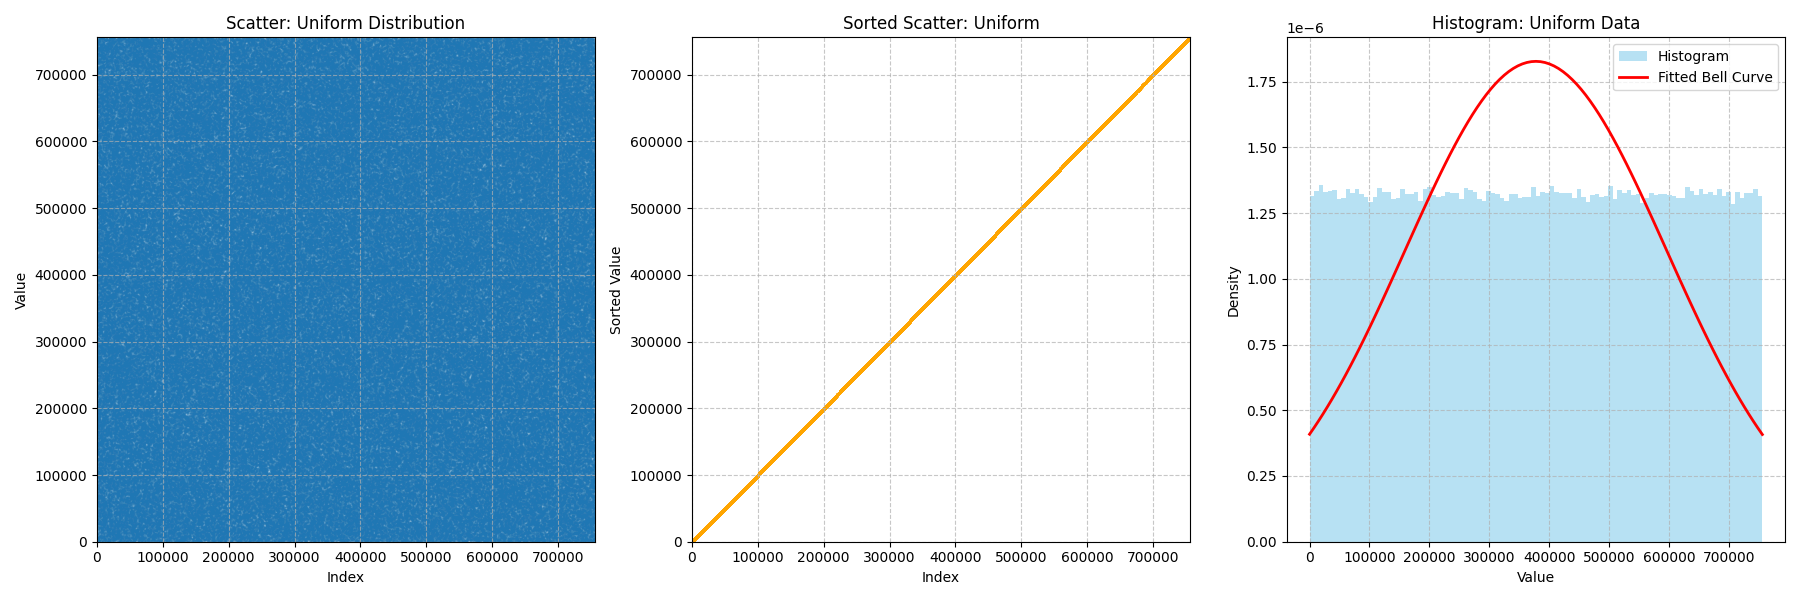
\includegraphics[width=0.8\textwidth]{src/out/1run_4node_4seed_uniform.png}
    \caption{Dataset distribution for Run 1 - Uniform, 4 Nodes, Seed 4}
    \label{fig:run1_dist}
\end{figure}

\textbf{Cluster \& Data:} 4 Nodes, Data Size = 756,000 elements.\\
\textbf{Sequential Baseline:} Time = 180,655.9 \textmu{}s, Throughput = 0.238963 \textmu{}s/element.

\begin{table}[H]
\centering
\caption{Performance metrics for Run 1}
\label{tab:run1}
\begin{tabular}{@{}lcc@{}}
\toprule
\textbf{Metric} & \textbf{H-PSRS} & \textbf{H-PSLP} \\
\midrule
\textbf{Makespan (\textmu{}s)} & 38,686.0 & \textbf{29,793.6} \\
\textbf{Total Cost (\$)} & 56,206.33 & \textbf{28,788.23} \\
\textbf{Preprocessing Overhead (\textmu{}s)} & 392.990 & 375.450 \\
\textbf{H-PSRS Memory Overflow} & N3 (425.4\%), N1 (233.9\%) & N/A \\
\textbf{H-PSLP Max Mem. Util.} & N/A & N1 (100.0\%) \\
\textbf{LP Model Predicted Makespan (sort) (\textmu{}s)} & N/A & \textbf{14,044.3} \\
\textbf{Actual Max Local Sort Time (\textmu{}s)} & N/A & 16,422.7 \\
\textbf{LP Model Predicted Cost (sort) (\$)} & N/A & \textbf{17,655.42} \\
\textbf{Actual Sum of Local Sort Costs (\$)} & N/A & 21,189.53 \\
\bottomrule
\end{tabular}
\end{table}

\subsubsection{Run 2: Uniform Distribution, 4 Nodes, Seed 5}

\begin{figure}[H]
    \centering
    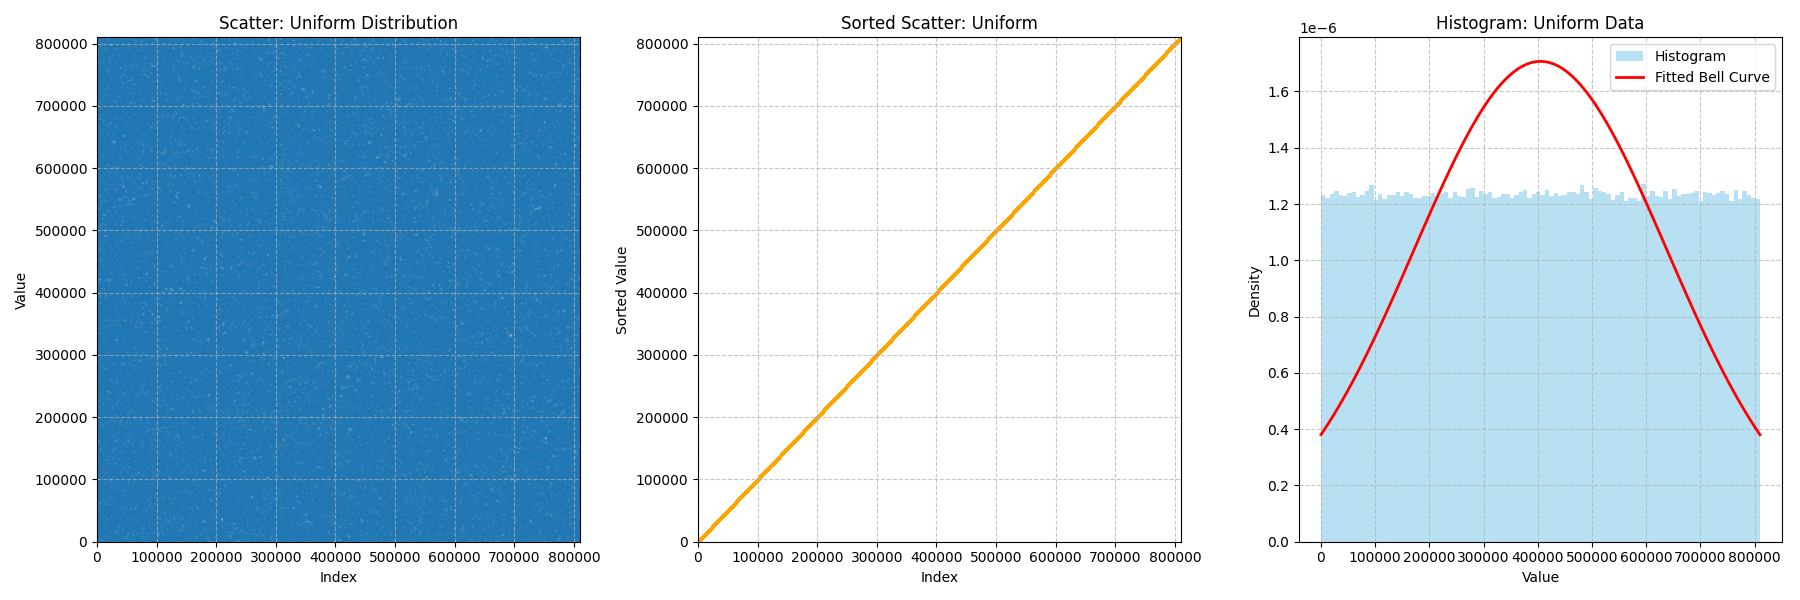
\includegraphics[width=0.8\textwidth]{src/out/2run_4node_5seed_uniform.png}
    \caption{Dataset distribution for Run 2 - Uniform, 4 Nodes, Seed 5}
    \label{fig:run2_dist}
\end{figure}

\textbf{Cluster \& Data:} 4 Nodes, Data Size = 810,000 elements.\\
\textbf{Sequential Baseline:} Time = 186,810.6 \textmu{}s, Throughput = 0.230630 \textmu{}s/element.

\begin{table}[H]
\centering
\caption{Performance metrics for Run 2}
\label{tab:run2}
\begin{tabular}{@{}lcc@{}}
\toprule
\textbf{Metric} & \textbf{H-PSRS} & \textbf{H-PSLP} \\
\midrule
\textbf{Makespan (\textmu{}s)} & 34,005.6 & \textbf{20,633.4} \\
\textbf{Total Cost (\$)} & 30,512.35 & \textbf{13,557.69} \\
\textbf{Preprocessing Overhead (\textmu{}s)} & 258.199 & 288.044 \\
\textbf{H-PSRS Memory Overflow} & N0 (1599.0\%) & N/A \\
\textbf{H-PSLP Max Mem. Util.} & N/A & N1 (99.8\%) \\
\textbf{LP Model Predicted Makespan (sort) (\textmu{}s)} & N/A & \textbf{9,145.8} \\
\textbf{Actual Max Local Sort Time (\textmu{}s)} & N/A & 9,790.4 \\
\textbf{LP Model Predicted Cost (sort) (\$)} & N/A & \textbf{9,921.22} \\
\textbf{Actual Sum of Local Sort Costs (\$)} & N/A & 10,049.08 \\
\bottomrule
\end{tabular}
\end{table}

\subsubsection{Run 3: Uniform Distribution, 8 Nodes, Seed 4}

\begin{figure}[H]
    \centering
    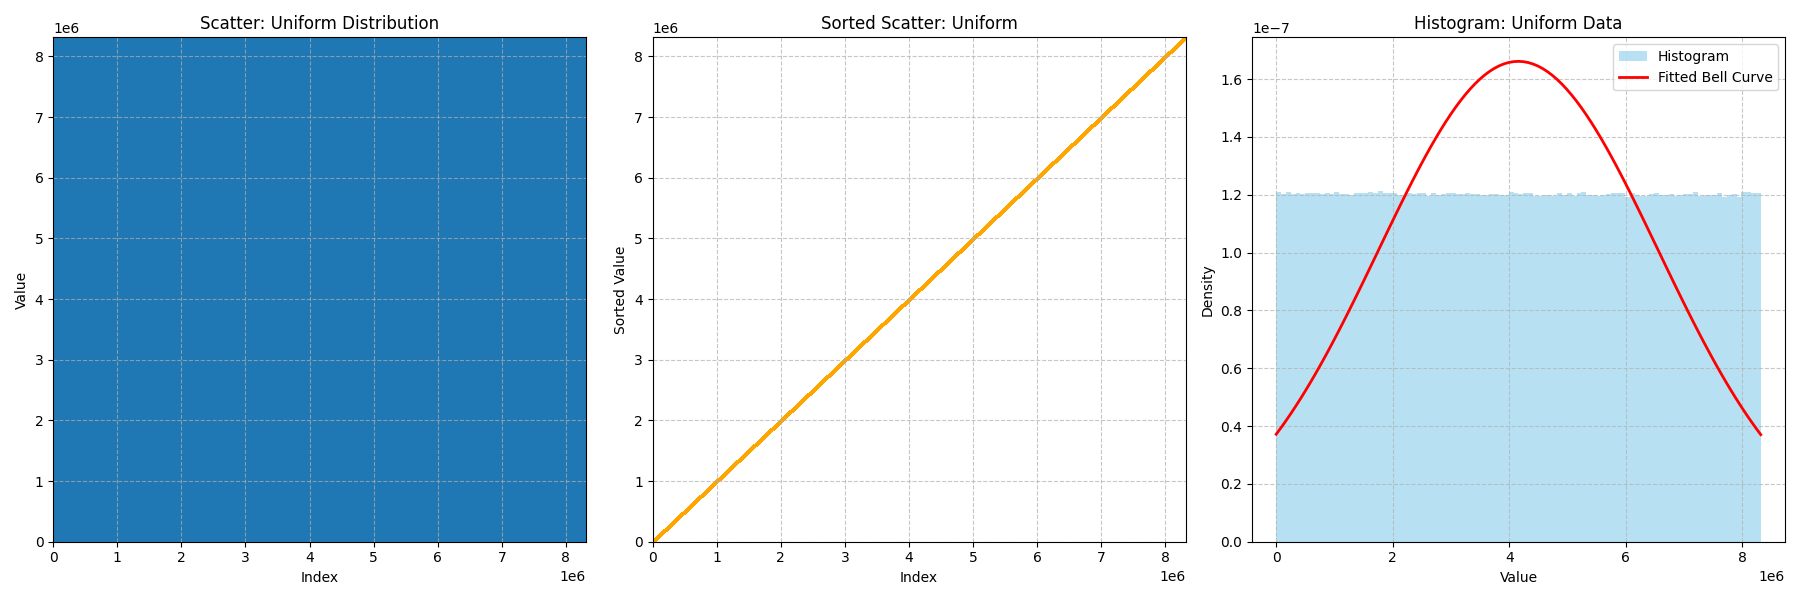
\includegraphics[width=0.8\textwidth]{src/out/3run_8node_4seed_uniform.png}
    \caption{Dataset distribution for Run 3 - Uniform, 8 Nodes, Seed 4}
    \label{fig:run3_dist}
\end{figure}

\textbf{Cluster \& Data:} 8 Nodes, Data Size = 8,316,000 elements.\\
\textbf{Sequential Baseline:} Time = 2,726,167.9 \textmu{}s, Throughput = 0.327822 \textmu{}s/element.

\begin{table}[H]
\centering
\caption{Performance metrics for Run 3}
\label{tab:run3}
\begin{tabular}{@{}lcc@{}}
\toprule
\textbf{Metric} & \textbf{H-PSRS} & \textbf{H-PSLP} \\
\midrule
\textbf{Makespan (\textmu{}s)} & 445,299.3 & \textbf{311,808.0} \\
\textbf{Total Cost (\$)} & 816,014.97 & \textbf{284,321.96} \\
\textbf{Preprocessing Overhead (\textmu{}s)} & 4635.303 & 8935.205 \\
\textbf{H-PSRS Memory Overflow} & N3 (1454.8\%), N0 (979.9\%) & N/A \\
\textbf{H-PSLP Max Mem. Util.} & N/A & N2 (99.7\%) \\
\textbf{LP Model Predicted Makespan (sort) (\textmu{}s)} & N/A & \textbf{125,524.1} \\
\textbf{Actual Max Local Sort Time (\textmu{}s)} & N/A & 122,323.7 \\
\textbf{LP Model Predicted Cost (sort) (\$)} & N/A & \textbf{303,521.59} \\
\textbf{Actual Sum of Local Sort Costs (\$)} & N/A & 274,580.60 \\
\bottomrule
\end{tabular}
\end{table}

\subsubsection{Run 4: Uniform Distribution, 8 Nodes, Seed 5}

\begin{figure}[H]
    \centering
    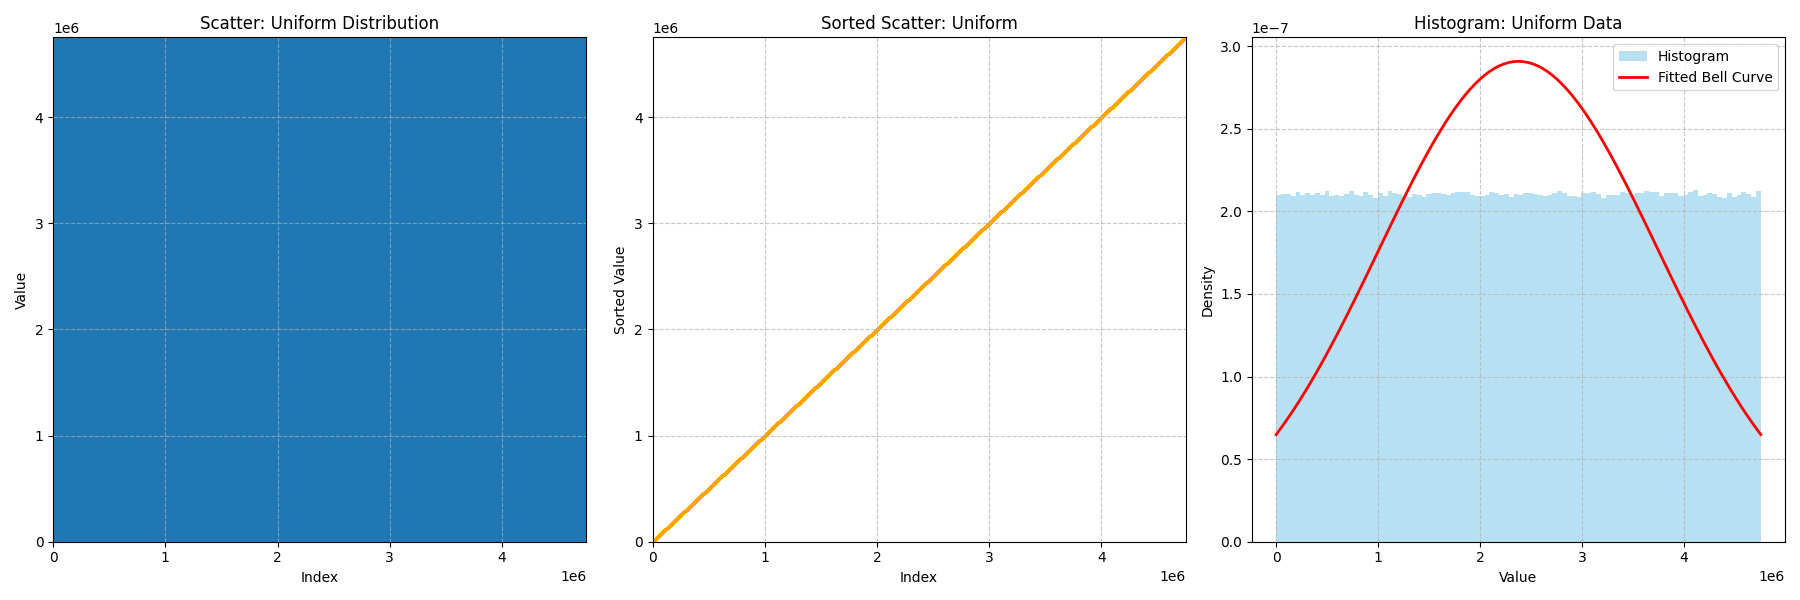
\includegraphics[width=0.8\textwidth]{src/out/4run_8node_5seed_uniform.png}
    \caption{Dataset distribution for Run 4 - Uniform, 8 Nodes, Seed 5}
    \label{fig:run4_dist}
\end{figure}

\textbf{Cluster \& Data:} 8 Nodes, Data Size = 4,752,000 elements.\\
\textbf{Sequential Baseline:} Time = 1,512,629.2 \textmu{}s, Throughput = 0.318314 \textmu{}s/element.

\begin{table}[H]
\centering
\caption{Performance metrics for Run 4}
\label{tab:run4}
\begin{tabular}{@{}lcc@{}}
\toprule
\textbf{Metric} & \textbf{H-PSRS} & \textbf{H-PSLP} \\
\midrule
\textbf{Makespan (\textmu{}s)} & 272,898.9 & \textbf{113,946.7} \\
\textbf{Total Cost (\$)} & 306,606.23 & \textbf{110,491.35} \\
\textbf{Preprocessing Overhead (\textmu{}s)} & 1610.111 & 361.807 \\
\textbf{H-PSRS Memory Overflow} & \begin{tabular}[c]{@{}l@{}}N4 (205.9\%),\\ N5 (1422.2\%),\\ N1 (170.2\%)\end{tabular} & N/A \\
\textbf{H-PSLP Max Mem. Util.} & N/A & N5 (100.1\%) \\
\textbf{LP Model Predicted Makespan (sort) (\textmu{}s)} & N/A & \textbf{47,603.4} \\
\textbf{Actual Max Local Sort Time (\textmu{}s)} & N/A & 43,836.4 \\
\textbf{LP Model Predicted Cost (sort) (\$)} & N/A & \textbf{136,047.90} \\
\textbf{Actual Sum of Local Sort Costs (\$)} & N/A & 87,424.32 \\
\bottomrule
\end{tabular}
\end{table}

\subsubsection{Run 5: Gaussian Distribution, 4 Nodes, Seed 4}

\begin{figure}[H]
    \centering
    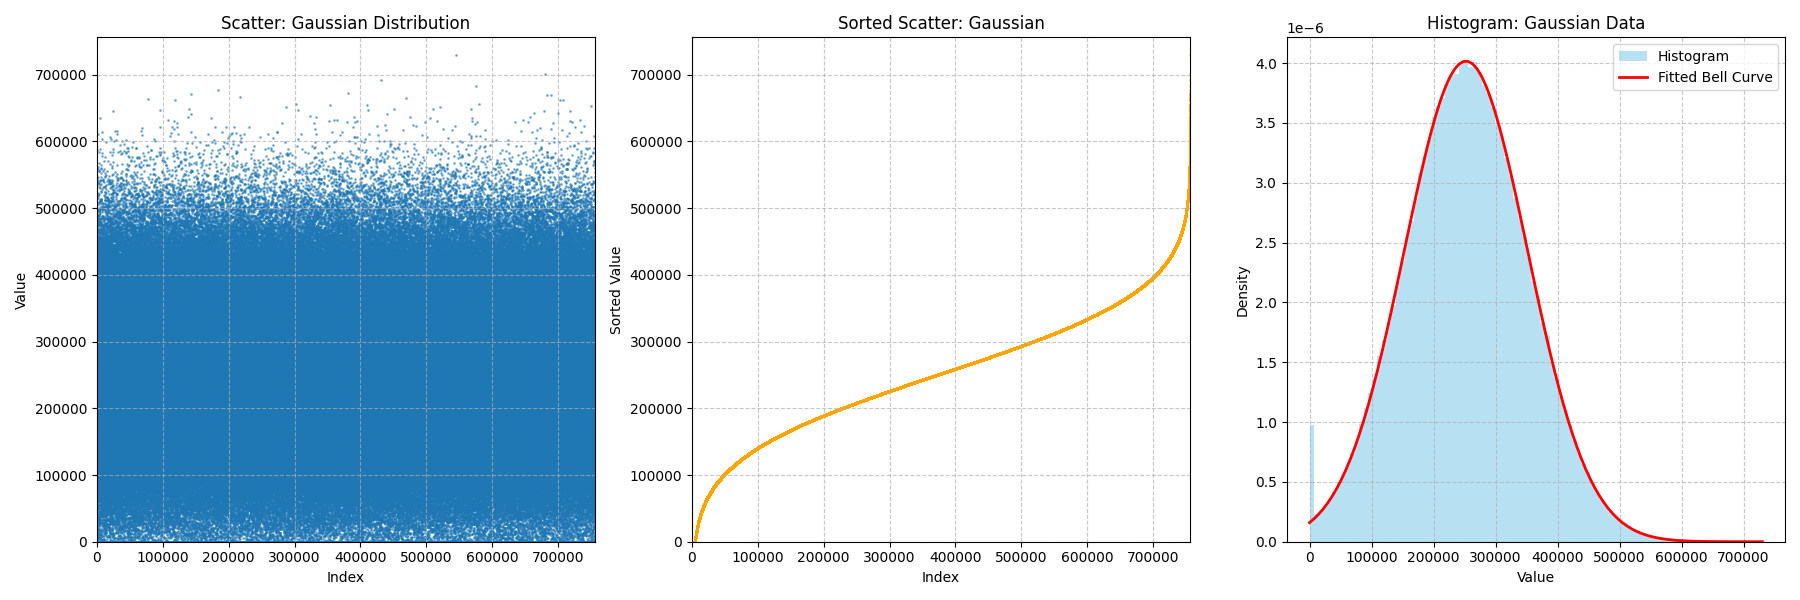
\includegraphics[width=0.8\textwidth]{src/out/5run_4node_4seed_gaussian.png}
    \caption{Dataset distribution for Run 5 - Gaussian (mean 252k, std 100k), 4 Nodes, Seed 4}
    \label{fig:run5_dist}
\end{figure}

\textbf{Cluster \& Data:} 4 Nodes, Data Size = 756,000 elements.\\
\textbf{Sequential Baseline:} Time = 178,218.0 \textmu{}s, Throughput = 0.235738 \textmu{}s/element.

\begin{table}[H]
\centering
\caption{Performance metrics for Run 5}
\label{tab:run5}
\begin{tabular}{@{}lcc@{}}
\toprule
\textbf{Metric} & \textbf{H-PSRS} & \textbf{H-PSLP} \\
\midrule
\textbf{Makespan (\textmu{}s)} & 40,108.8 & \textbf{30,114.0} \\
\textbf{Total Cost (\$)} & 54,000.01 & \textbf{26,420.90} \\
\textbf{Preprocessing Overhead (\textmu{}s)} & 334.683 & 477.432 \\
\textbf{H-PSRS Memory Overflow} & N3 (425.4\%), N1 (233.9\%) & N/A \\
\textbf{H-PSLP Max Mem. Util.} & N/A & N1 (100.0\%) \\
\textbf{LP Model Predicted Makespan (sort) (\textmu{}s)} & N/A & \textbf{13,854.7} \\
\textbf{Actual Max Local Sort Time (\textmu{}s)} & N/A & 18,009.5 \\
\textbf{LP Model Predicted Cost (sort) (\$)} & N/A & \textbf{17,417.16} \\
\textbf{Actual Sum of Local Sort Costs (\$)} & N/A & 21,842.52 \\
\bottomrule
\end{tabular}
\end{table}

\subsubsection{Run 6: Gaussian Distribution, 4 Nodes, Seed 5}

\begin{figure}[H]
    \centering
    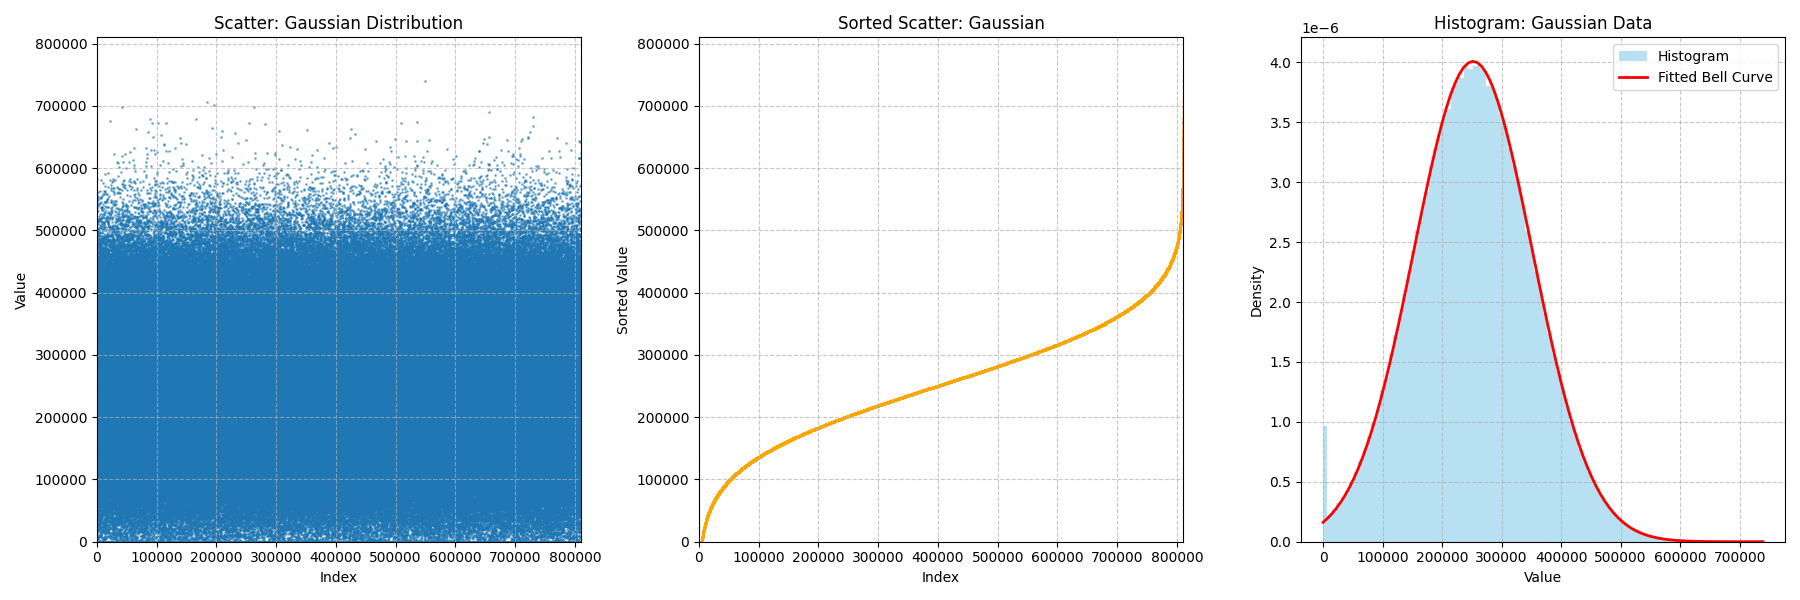
\includegraphics[width=0.8\textwidth]{src/out/6run_4node_5seed_gaussian.png}
    \caption{Dataset distribution for Run 6 - Gaussian (mean 252k, std 100k), 4 Nodes, Seed 5}
    \label{fig:run6_dist}
\end{figure}

\textbf{Cluster \& Data:} 4 Nodes, Data Size = 810,000 elements.\\
\textbf{Sequential Baseline:} Time = 195,203.4 \textmu{}s, Throughput = 0.240992 \textmu{}s/element.

\begin{table}[H]
\centering
\caption{Performance metrics for Run 6}
\label{tab:run6}
\begin{tabular}{@{}lcc@{}}
\toprule
\textbf{Metric} & \textbf{H-PSRS} & \textbf{H-PSLP} \\
\midrule
\textbf{Makespan (\textmu{}s)} & 36,290.1 & \textbf{22,019.5} \\
\textbf{Total Cost (\$)} & 33,712.17 & \textbf{12,447.08} \\
\textbf{Preprocessing Overhead (\textmu{}s)} & 323.418 & 313.903 \\
\textbf{H-PSRS Memory Overflow} & N0 (1599.0\%) & N/A \\
\textbf{H-PSLP Max Mem. Util.} & N/A & N1 (99.8\%) \\
\textbf{LP Model Predicted Makespan (sort) (\textmu{}s)} & N/A & \textbf{9,556.7} \\
\textbf{Actual Max Local Sort Time (\textmu{}s)} & N/A & 11,038.9 \\
\textbf{LP Model Predicted Cost (sort) (\$)} & N/A & \textbf{10,366.95} \\
\textbf{Actual Sum of Local Sort Costs (\$)} & N/A & 12,135.29 \\
\bottomrule
\end{tabular}
\end{table}

\subsubsection{Run 7: Gaussian Distribution, 8 Nodes, Seed 4}

\begin{figure}[H]
    \centering
    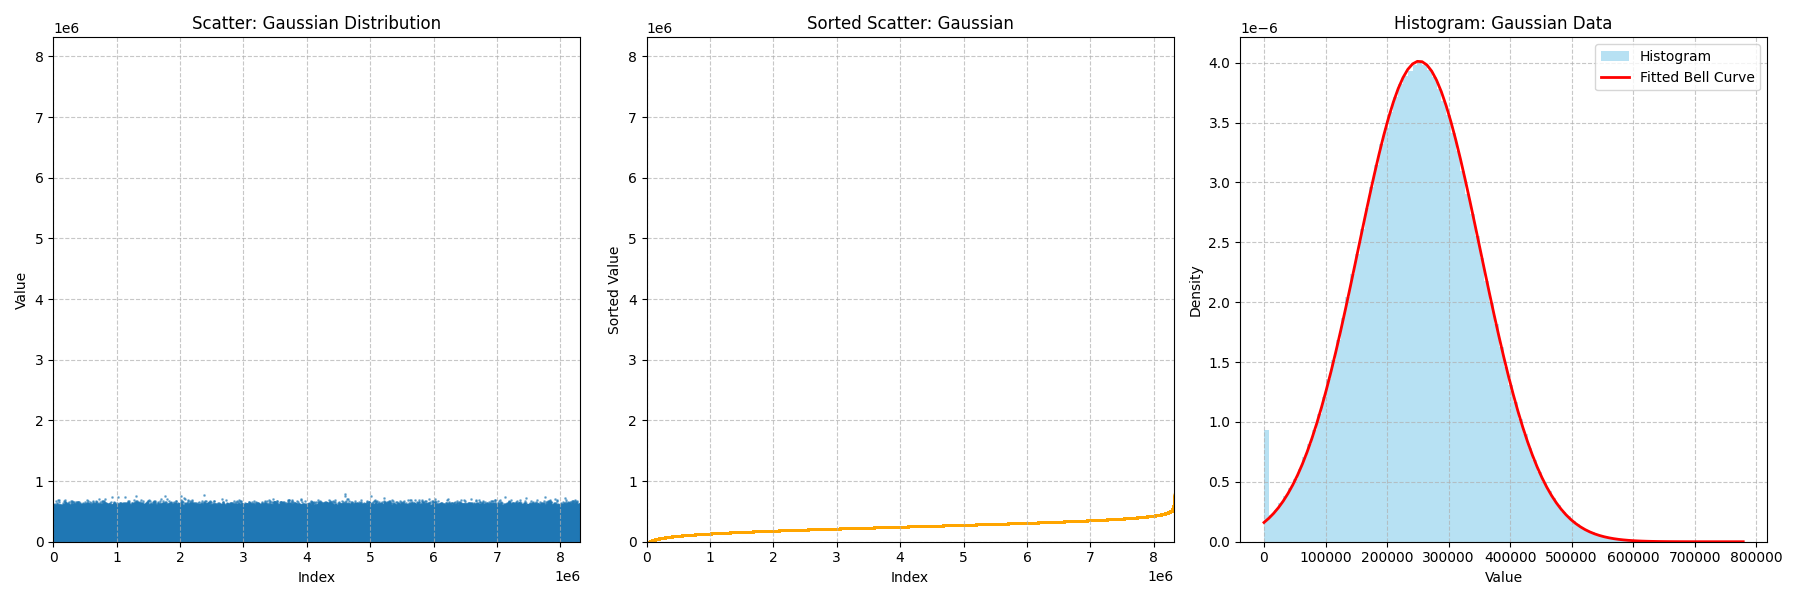
\includegraphics[width=0.8\textwidth]{src/out/7run_8node_4seed_gaussian.png}
    \caption{Dataset distribution for Run 7 - Gaussian (mean 252k, std 100k), 8 Nodes, Seed 4}
    \label{fig:run7_dist}
\end{figure}

\textbf{Cluster \& Data:} 8 Nodes, Data Size = 8,316,000 elements.\\
\textbf{Sequential Baseline:} Time = 2,850,812.1 \textmu{}s, Throughput = 0.342810 \textmu{}s/element.

\begin{table}[H]
\centering
\caption{Performance metrics for Run 7}
\label{tab:run7}
\begin{tabular}{@{}lcc@{}}
\toprule
\textbf{Metric} & \textbf{H-PSRS} & \textbf{H-PSLP} \\
\midrule
\textbf{Makespan (\textmu{}s)} & 446,139.2 & \textbf{319,017.1} \\
\textbf{Total Cost (\$)} & 839,765.87 & \textbf{292,759.19} \\
\textbf{Preprocessing Overhead (\textmu{}s)} & 5090.880 & 8935.205 \\
\textbf{H-PSRS Memory Overflow} & N3 (1454.8\%), N0 (979.9\%) & N/A \\
\textbf{H-PSLP Max Mem. Util.} & N/A & N2 (99.7\%) \\
\textbf{LP Model Predicted Makespan (sort) (\textmu{}s)} & N/A & \textbf{125,524.1} \\
\textbf{Actual Max Local Sort Time (\textmu{}s)} & N/A & 122,323.7 \\
\textbf{LP Model Predicted Cost (sort) (\$)} & N/A & \textbf{303,521.59} \\
\textbf{Actual Sum of Local Sort Costs (\$)} & N/A & 274,580.60 \\
\bottomrule
\end{tabular}
\end{table}

\subsubsection{Run 8: Gaussian Distribution, 8 Nodes, Seed 5}

\begin{figure}[H]
    \centering
    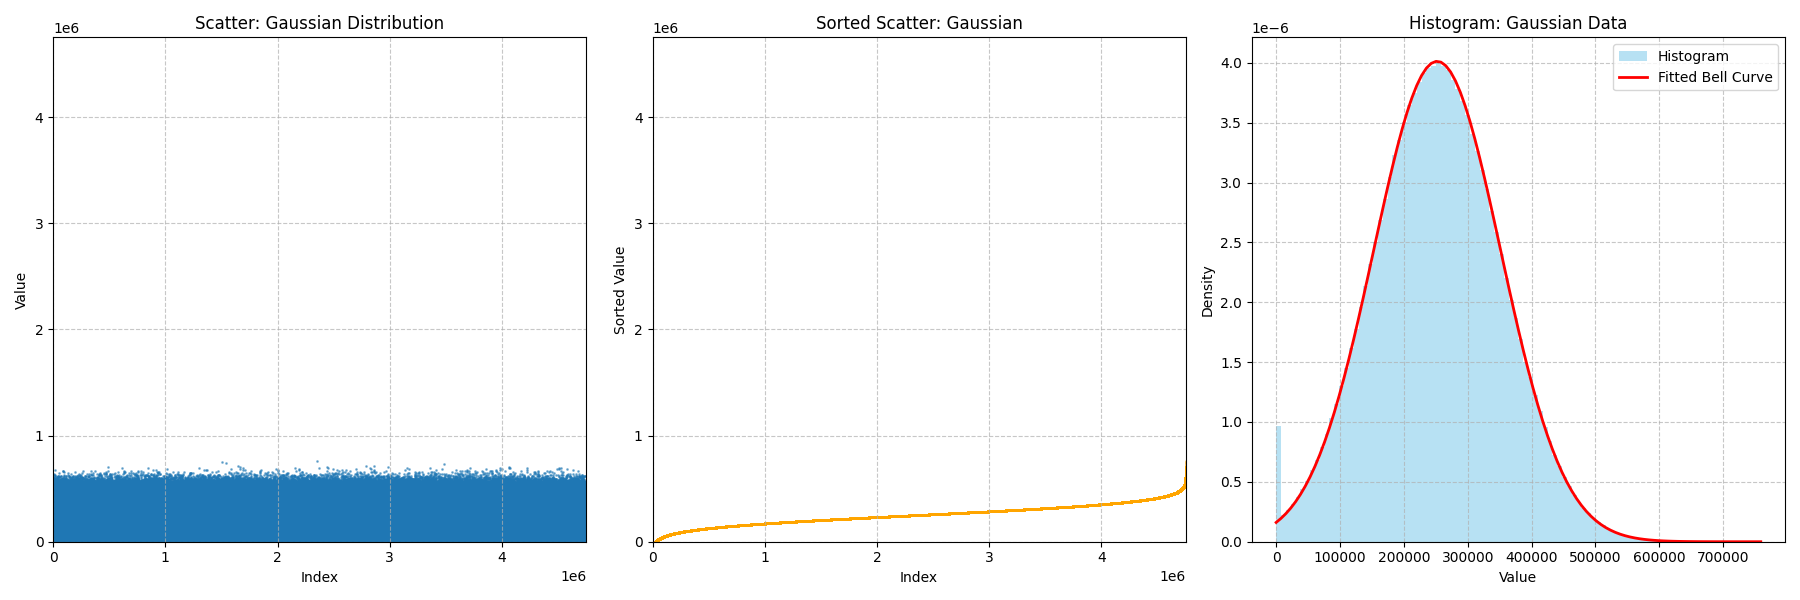
\includegraphics[width=0.8\textwidth]{src/out/8run_8node_5seed_gaussian.png}
    \caption{Dataset distribution for Run 8 - Gaussian (mean 252k, std 100k), 8 Nodes, Seed 5}
    \label{fig:run8_dist}
\end{figure}

\textbf{Cluster \& Data:} 8 Nodes, Data Size = 4,752,000 elements.\\
\textbf{Sequential Baseline:} Time = 1,540,436.0 \textmu{}s, Throughput = 0.324166 \textmu{}s/element.

\begin{table}[H]
\centering
\caption{Performance metrics for Run 8}
\label{tab:run8}
\begin{tabular}{@{}lcc@{}}
\toprule
\textbf{Metric} & \textbf{H-PSRS} & \textbf{H-PSLP} \\
\midrule
\textbf{Makespan (\textmu{}s)} & 178,432.2 & \textbf{124,284.2} \\
\textbf{Total Cost (\$)} & 428,716.62 & \textbf{154,602.50} \\
\textbf{Preprocessing Overhead (\textmu{}s)} & 2432.684 & 261.470 \\
\textbf{H-PSRS Memory Overflow} & \begin{tabular}[c]{@{}l@{}}N5 (1422.2\%),\\ N4 (205.9\%),\\ N1 (170.2\%)\end{tabular} & N/A \\
\textbf{H-PSLP Max Mem. Util.} & N/A & N5 (100.1\%) \\
\textbf{LP Model Predicted Makespan (sort) (\textmu{}s)} & N/A & \textbf{48,478.5} \\
\textbf{Actual Max Local Sort Time (\textmu{}s)} & N/A & 44,617.9 \\
\textbf{LP Model Predicted Cost (sort) (\$)} & N/A & \textbf{138,548.89} \\
\textbf{Actual Sum of Local Sort Costs (\$)} & N/A & 126,599.78 \\
\bottomrule
\end{tabular}
\end{table}

\subsection{Aggregated Results and Averages}

For configurations with two seeds, we calculate averages and standard deviations (StdDev).

\subsubsection{Configuration: Uniform Distribution, 4 Nodes (Runs 1 \& 2)}

\begin{table}[H]
\centering
\caption{Aggregated results for Uniform Distribution, 4 Nodes}
\label{tab:agg_uniform_4}
\begin{tabular}{@{}lcc@{}}
\toprule
\textbf{Metric (Avg ± StdDev)} & \textbf{H-PSRS} & \textbf{H-PSLP} \\
\midrule
\textbf{Makespan (\textmu{}s)} & 36,345.8 ± 3,309.6 & \textbf{25,213.5 ± 6,477.2} \\
\textbf{Total Cost (\$)} & 43,359.34 ± 18,168.4 & \textbf{21,172.96 ± 10,769.7} \\
\bottomrule
\end{tabular}
\end{table}

\subsubsection{Configuration: Uniform Distribution, 8 Nodes (Runs 3 \& 4)}

\begin{table}[H]
\centering
\caption{Aggregated results for Uniform Distribution, 8 Nodes}
\label{tab:agg_uniform_8}
\begin{tabular}{@{}lcc@{}}
\toprule
\textbf{Metric (Avg ± StdDev)} & \textbf{H-PSRS} & \textbf{H-PSLP} \\
\midrule
\textbf{Makespan (\textmu{}s)} & 359,099.1 ± 121,907.0 & \textbf{212,877.4 ± 139,910.0} \\
\textbf{Total Cost (\$)} & 561,310.60 ± 360,210.0 & \textbf{197,406.66 ± 123,000.0} \\
\bottomrule
\end{tabular}
\end{table}

\subsubsection{Configuration: Gaussian Distribution, 4 Nodes (Runs 5 \& 6)}

\begin{table}[H]
\centering
\caption{Aggregated results for Gaussian Distribution, 4 Nodes}
\label{tab:agg_gaussian_4}
\begin{tabular}{@{}lcc@{}}
\toprule
\textbf{Metric (Avg ± StdDev)} & \textbf{H-PSRS} & \textbf{H-PSLP} \\
\midrule
\textbf{Makespan (\textmu{}s)} & 38,199.5 ± 2,693.0 & \textbf{26,066.8 ± 5,724.1} \\
\textbf{Total Cost (\$)} & 43,856.09 ± 14,345.6 & \textbf{19,433.99 ± 9,881.1} \\
\bottomrule
\end{tabular}
\end{table}

\subsubsection{Configuration: Gaussian Distribution, 8 Nodes (Runs 7 \& 8)}

\begin{table}[H]
\centering
\caption{Aggregated results for Gaussian Distribution, 8 Nodes}
\label{tab:agg_gaussian_8}
\begin{tabular}{@{}lcc@{}}
\toprule
\textbf{Metric (Avg ± StdDev)} & \textbf{H-PSRS} & \textbf{H-PSLP} \\
\midrule
\textbf{Makespan (\textmu{}s)} & 312,285.7 ± 189,297.0 & \textbf{221,650.7 ± 137,700.0} \\ 
\textbf{Total Cost (\$)} & 634,241.25 ± 290,650.0 & \textbf{223,680.85 ± 97,691.0} \\ 
\bottomrule
\end{tabular}
\end{table}

\subsection{Visual Performance Comparisons}
\label{sec:visual_perf}

The following charts visually summarize the performance comparisons based on the aggregated experimental data and specific run examples.

\begin{figure}[H]
    \centering
    \begin{subfigure}{0.48\textwidth}
        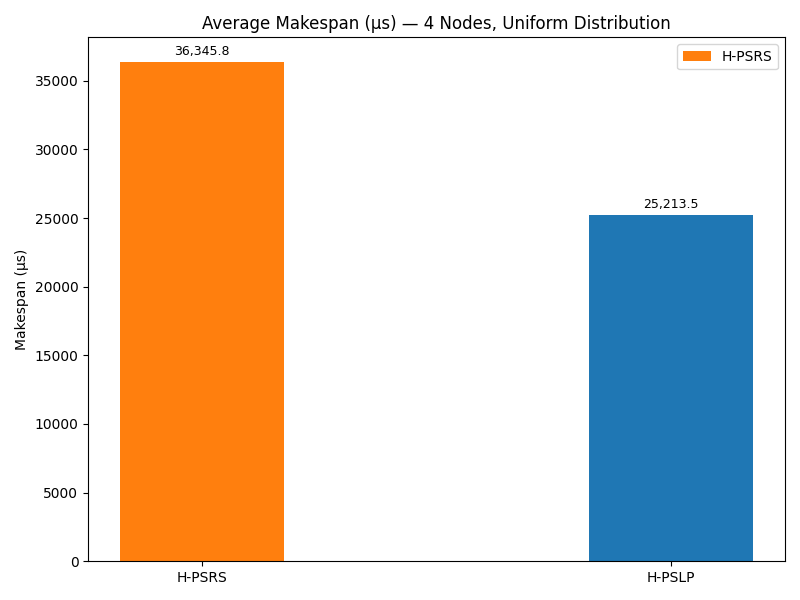
\includegraphics[width=\textwidth]{src/out_matplotlib_charts/perf_makespan_uniform_4nodes.png}
        \caption{Makespan - Uniform, 4 Nodes}
        \label{fig:m1}
    \end{subfigure}
    \hfill
    \begin{subfigure}{0.48\textwidth}
        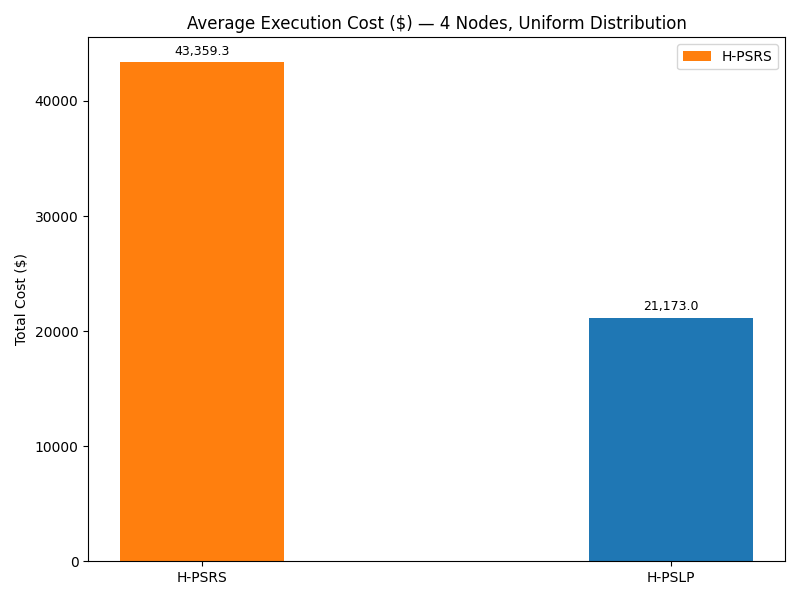
\includegraphics[width=\textwidth]{src/out_matplotlib_charts/perf_cost_uniform_4nodes.png}
        \caption{Cost - Uniform, 4 Nodes}
        \label{fig:m2}
    \end{subfigure}
    \caption{Performance Comparison: Uniform Data, 4 Nodes (Average)}
    \label{fig:perf_uniform_4nodes}
\end{figure}

\begin{figure}[H]
    \centering
    \begin{subfigure}{0.48\textwidth}
        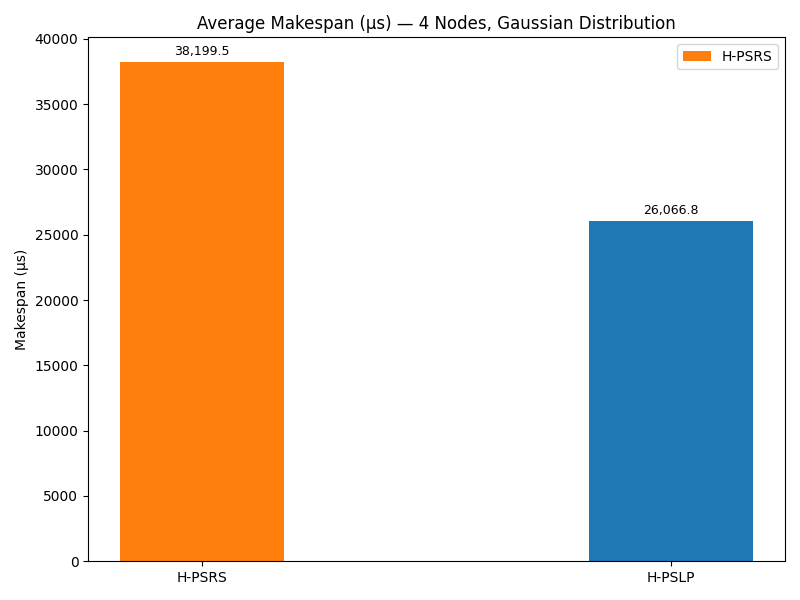
\includegraphics[width=\textwidth]{src/out_matplotlib_charts/perf_makespan_gaussian_4nodes.png}
        \caption{Makespan - Gaussian, 4 Nodes}
        \label{fig:m3}
    \end{subfigure}
    \hfill
    \begin{subfigure}{0.48\textwidth}
        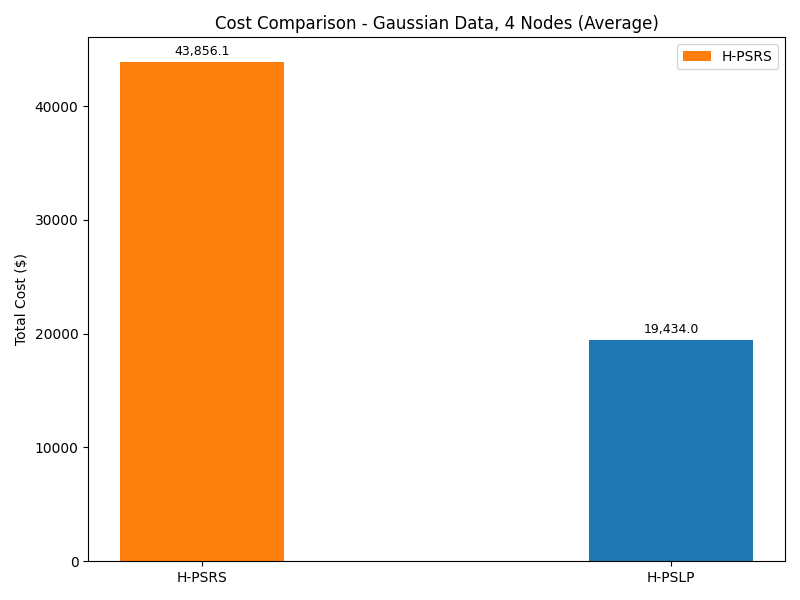
\includegraphics[width=\textwidth]{src/out_matplotlib_charts/perf_cost_gaussian_4nodes.png}
        \caption{Cost - Gaussian, 4 Nodes}
        \label{fig:m4}
    \end{subfigure}
    \caption{Performance Comparison: Gaussian Data, 4 Nodes (Average)}
    \label{fig:perf_gaussian_4nodes}
\end{figure}

\begin{figure}[H]
    \centering
    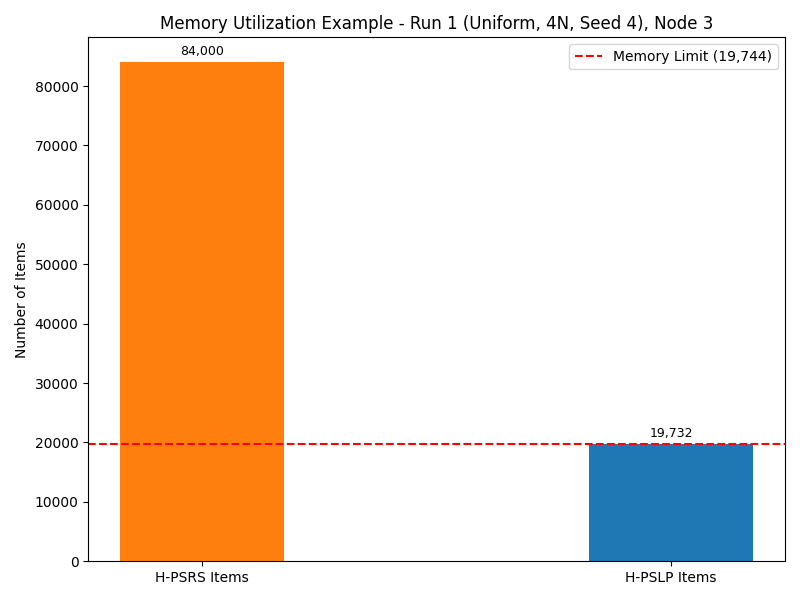
\includegraphics[width=0.6\textwidth]{src/out_matplotlib_charts/perf_memory_util_example.png}
    \caption{Memory Utilization Example - Run 1, Node 3}
    \label{fig:m5}
\end{figure}

\begin{figure}[H]
    \centering
    \begin{subfigure}{0.48\textwidth}
        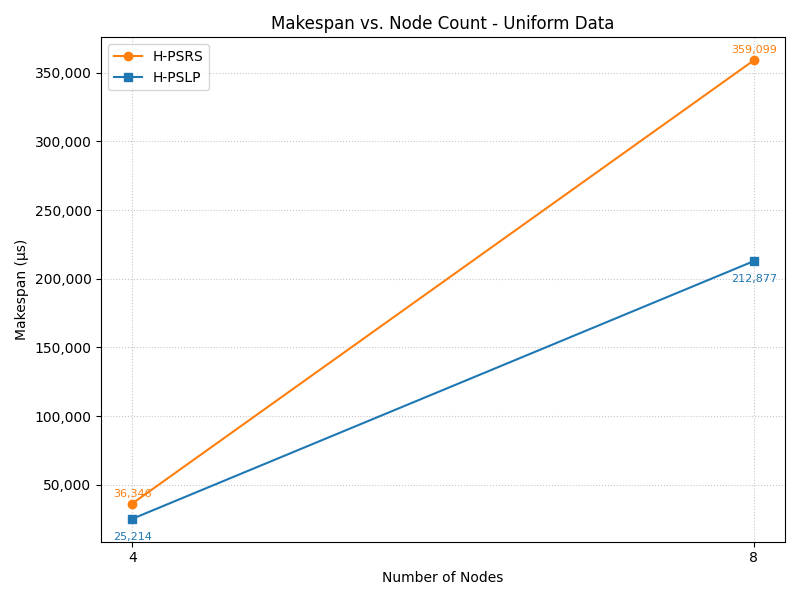
\includegraphics[width=\textwidth]{src/out_matplotlib_charts/scale_makespan_uniform_nodes.png}
        \caption{Makespan vs. Node Count}
        \label{fig:m6}
    \end{subfigure}
    \hfill
    \begin{subfigure}{0.48\textwidth}
        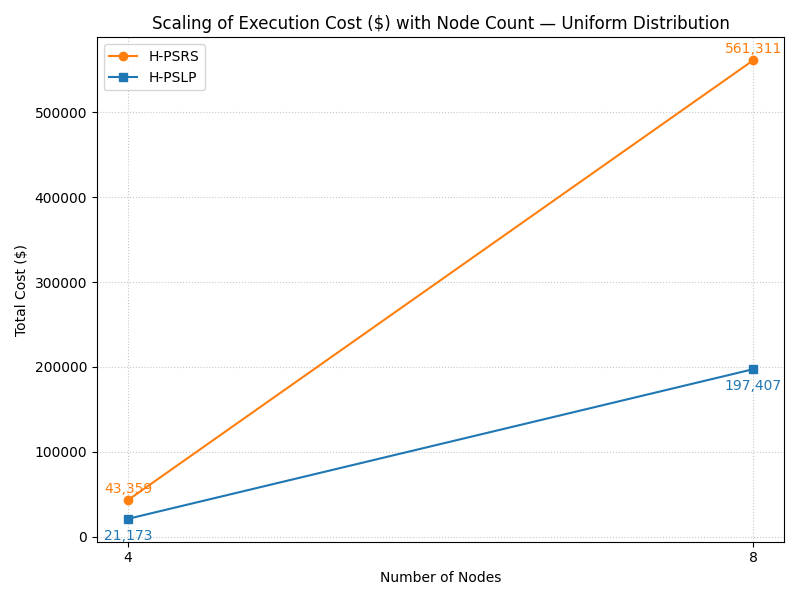
\includegraphics[width=\textwidth]{src/out_matplotlib_charts/scale_cost_uniform_nodes.png}
        \caption{Cost vs. Node Count}
        \label{fig:m7}
    \end{subfigure}
    \caption{Scalability Analysis: Uniform Data}
    \label{fig:scale_uniform}
\end{figure}

\begin{figure}[H]
    \centering
    \begin{subfigure}{0.48\textwidth}
        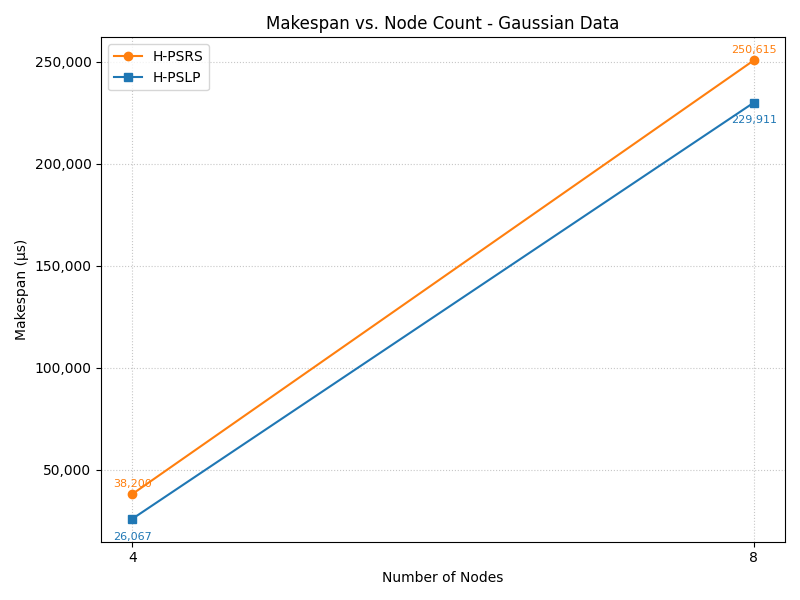
\includegraphics[width=\textwidth]{src/out_matplotlib_charts/scale_makespan_gaussian_nodes.png}
        \caption{Makespan vs. Node Count}
        \label{fig:m8}
    \end{subfigure}
    \hfill
    \begin{subfigure}{0.48\textwidth}
        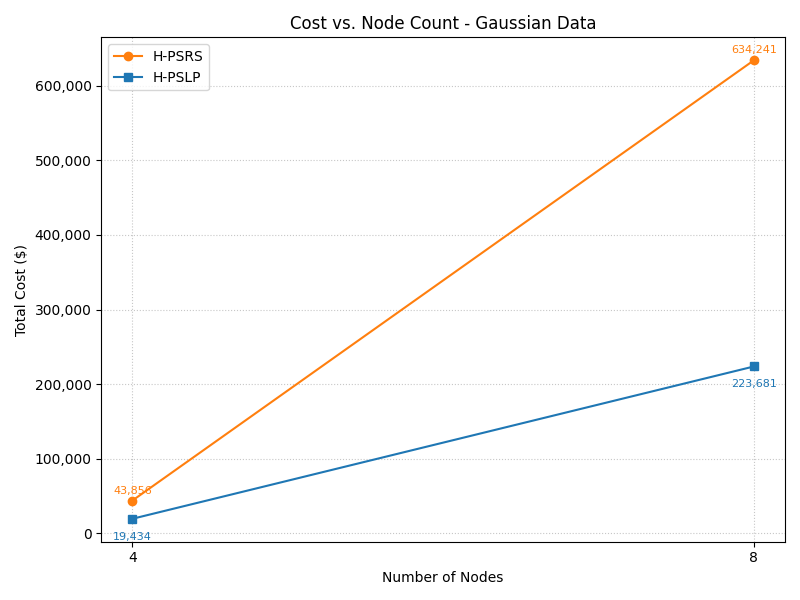
\includegraphics[width=\textwidth]{src/out_matplotlib_charts/scale_cost_gaussian_nodes.png}
        \caption{Cost vs. Node Count}
        \label{fig:m9}
    \end{subfigure}
    \caption{Scalability Analysis: Gaussian Data}
    \label{fig:scale_gaussian}
\end{figure}

\begin{figure}[H]
    \centering
    \begin{subfigure}{0.48\textwidth}
        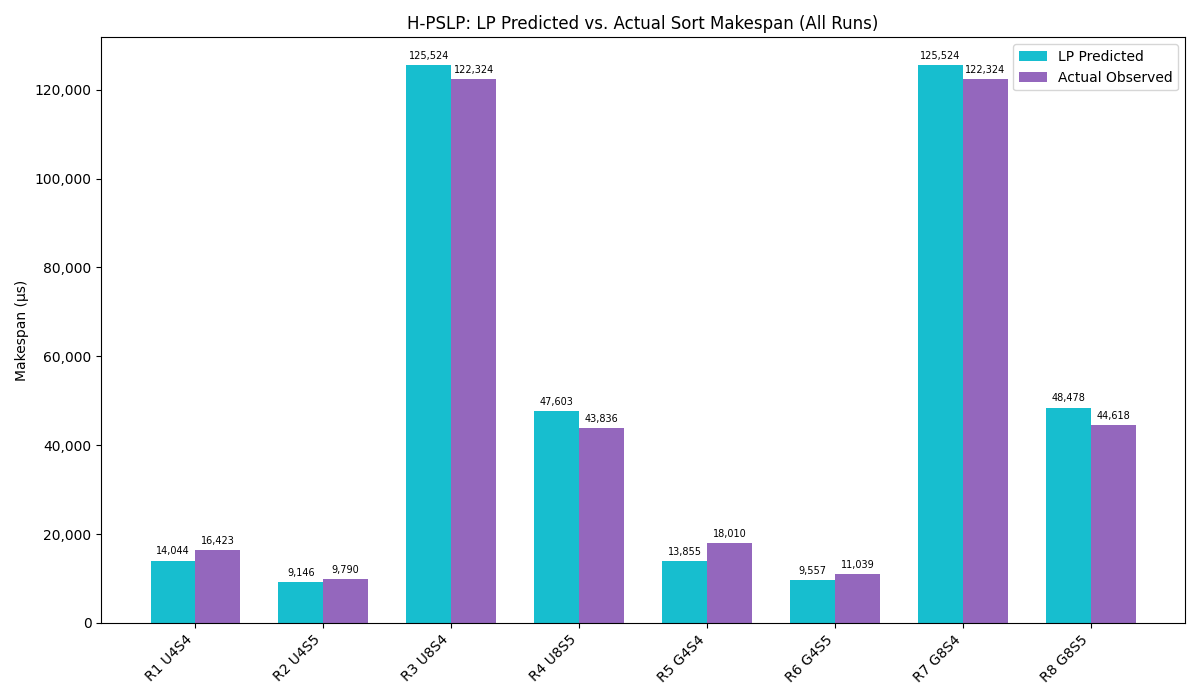
\includegraphics[width=\textwidth]{src/out_matplotlib_charts/pred_vs_actual_makespan_hpslp.png}
        \caption{Predicted vs. Actual Sort Makespan}
        \label{fig:m10}
    \end{subfigure}
    \hfill
    \begin{subfigure}{0.48\textwidth}
        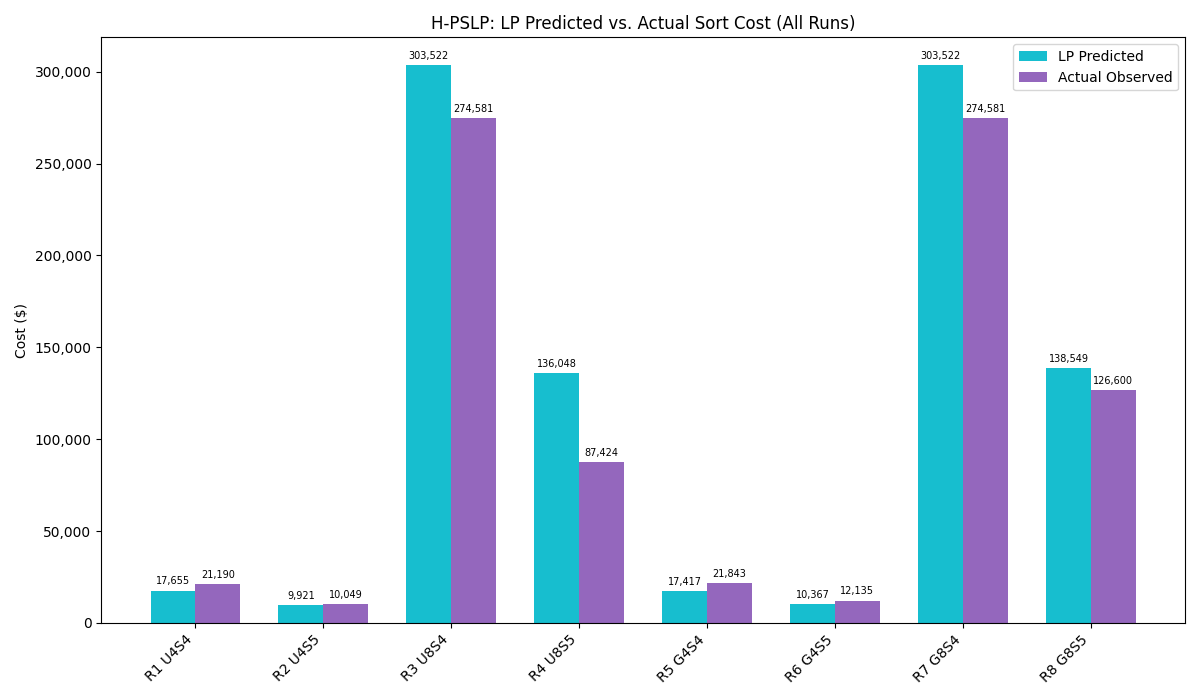
\includegraphics[width=\textwidth]{src/out_matplotlib_charts/pred_vs_actual_cost_hpslp.png}
        \caption{Predicted vs. Actual Sort Cost}
        \label{fig:m11}
    \end{subfigure}
    \caption{H-PSLP LP Model Prediction Accuracy for Sort Phase (All Runs)}
    \label{fig:pred_vs_actual}
\end{figure}

\section{Discussion}

The comprehensive simulation results across various configurations provide significant insights into the comparative performance of the sequential baseline, the Regular Sampling approach (H-PSRS), and the Static Optimized approach (H-PSLP).

\subsection{Key Findings Summary}
\begin{enumerate}
    \item \textbf{Superior Efficiency of H-PSLP:} Across the eight experimental runs, H-PSLP (Min-Heap Merge) demonstrated a significant performance advantage, reducing \textbf{makespan by an average of 33.3\%} and \textbf{total cost by an average of 60.7\%} compared to H-PSRS.
    
    \textit{Sample Speedup (Run 1: Uniform, 4 Nodes, Seed 4, vs. Sequential Baseline):}
    \begin{itemize}
        \item H-PSRS: 4.67$\times$
        \item H-PSLP: 6.06$\times$
    \end{itemize}

    \item \textbf{Elimination of Communication Bottlenecks:} H-PSLP’s static partitioning strategy entirely removes the costly all-to-all data redistribution phase inherent in H-PSRS. This directly translated to makespan savings. For instance, in Run 3 (8 nodes, uniform), the H-PSRS data partition and transfer phase contributed 158,639.4 \textmu{}s (Max Node Time) to its makespan; this component is absent in H-PSLP.

    \item \textbf{Guaranteed Memory Constraint Adherence:} A critical differentiator, H-PSLP consistently operated within node memory limits in all runs due to its LP formulation. In contrast, H-PSRS exhibited severe memory overflows in every run (e.g., Node 3 in Run 1 at 425.4\% overload; Node 0 in Run 2 at 1599.0\% overload), rendering it unreliable in memory-constrained scenarios.

    \item \textbf{Efficient Scalability with Low LP Overhead:} H-PSLP demonstrated good scalability. The LP solver overhead (a form of preprocessing) remained minimal, constituting a small fraction of the total makespan even with 8 nodes (e.g., 2.86\% of H-PSLP makespan in Run 3, 0.21\% in Run 8). Similarly, H-PSRS's initial partitioning overhead was also typically small relative to its overall makespan.

    \item \textbf{Robustness to Data Distribution:} H-PSLP performed consistently across uniform and Gaussian datasets. Average speedups (vs. sequential) for H-PSLP were 7.29$\times$ for uniform data (4-node) and 9.85$\times$ (8-node), and for Gaussian data were 7.16$\times$ (4-node) and 9.51$\times$ (8-node). H-PSRS achieved 5.05$\times$ (uniform 4-node), 5.43$\times$ (uniform 8-node), 4.89$\times$ (Gaussian 4-node), and 6.91$\times$ (Gaussian 8-node).
\end{enumerate}

\subsection{Overall Performance (Makespan and Cost)}

As highlighted in the Key Findings, the Static Optimized approach (H-PSLP) with Min-Heap Merge consistently outperformed H-PSRS.

\textbf{Makespan:} The average makespan reduction of 33.3\% by H-PSLP over H-PSRS indicates a substantial improvement in processing speed. For 4-node configurations, H-PSLP was approximately 30.1% faster on average. For 8-node configurations, H-PSLP was approximately 36.5% faster on average for uniform data and 28.4% faster for Gaussian data.

\textbf{Cost:} The average total cost reduction of 60.7\% by H-PSLP compared to H-PSRS is a compelling demonstration of its cost-aware optimization capabilities.

Solver and Initial Partitioning Overhead\subsection{Impact of Data Distribution (Uniform vs. Gaussian)}

Comparing runs with uniform distribution against Gaussian distribution (mean 252k, std 100k) for similar hardware configurations:

\textbf{H-PSRS Performance:} While makespan and cost for H-PSRS did not show dramatic average differences between the two distributions in 4-node setups, its reliance on pivot selection makes it inherently more sensitive to data skew. The critical issue of memory overflow remained regardless of the distribution.

\textbf{H-PSLP Performance:} H-PSLP's performance was consistently strong across both distributions. This robustness stems from its partitioning strategy being based on node capabilities and LP optimization, rather than data sampling.

\subsection{Impact of Node Count (4 Nodes vs. 8 Nodes)}

Increasing the number of nodes from 4 to 8:

\textbf{Scalability of Makespan:} While makespans increased for both methods with larger datasets on 8 nodes, H-PSLP's relative advantage over H-PSRS generally widened, suggesting better scalability.

\textbf{Cost Implications:} Total costs naturally increased with more nodes and larger datasets. However, H-PSLP's ability to optimize allocation continued to yield significant cost savings compared to H-PSRS, even with more nodes.

\textbf{Memory Overflows in H-PSRS:} The memory overflow problem in H-PSRS persisted and, in some 8-node cases (e.g., Run 3, Run 4, Run 8), affected multiple nodes, including high-throughput ones, due to the initial proportional allocation. This highlights a critical scalability flaw for H-PSRS in memory-constrained heterogeneous environments.

\subsection{Memory Management – A Decisive Factor}

This remains the most striking difference:

\textbf{H-PSRS:} Suffered severe memory overflows in every run, making it impractical for real-world systems where memory is a hard constraint.

\textbf{H-PSLP:} Successfully operated within all memory limits in every run, ensuring stability and reliability.

\subsection{Effectiveness of the LP Solver in H-PSLP}

The LP solver in H-PSLP consistently found efficient data distributions.

\textbf{Makespan \& Cost Prediction vs. Actual (for sort phase):} The LP model provides estimates for the makespan and cost of the parallel sorting phase. Visualizations (Figures~\ref{fig:m10} and \ref{fig:m11}) illustrate the comparison between these predictions and the actual observed metrics (Max Local Sort Time for makespan, Sum of Local Sort Costs for cost) across all runs.
\begin{itemize}
    \item For makespan, the predicted values were often close to the actuals. For example, in Run 3 (8 nodes, uniform), the predicted makespan for the sort phase was 125,524.1 \textmu{}s, and the actual maximum local sort time was 122,323.7 \textmu{}s (a difference of -2.6\%). In Run 8 (8 nodes, Gaussian), predicted was 48,478.5 \textmu{}s vs. actual 44,617.9 \textmu{}s (a difference of -8.6\%).
    \item For cost, differences were more varied. In Run 1 (4 nodes, uniform), the predicted sort phase cost was \$17,655.42, while the actual sum of local sort costs was \$21,189.53 (actual was 19.9\% higher). In Run 8, predicted sort cost was \$138,548.89, while actual was \$126,599.78 (actual was 8.6\% lower). These variations highlight that while the LP model effectively guides partitioning for good performance, its cost predictions for the sort phase can deviate due to simplifications (e.g., the \texttt{base\_throughput} factor) and uncaptured non-linear system behaviors. However, the overall H-PSLP approach (including solver and merge costs) still resulted in substantially lower total costs than H-PSRS.
\end{itemize}

\textbf{Solver and Initial Partitioning Overhead:} The preprocessing overhead, which includes the LP solver time for H-PSLP and the initial coordinator partitioning time for H-PSRS, was generally small compared to the overall makespan. For H-PSLP, the solver time typically constituted less than 1\% of its makespan for 4-node runs and under 3\% for 8-node runs (e.g., 2.86\% in Run 3, 0.21\% in Run 8). For H-PSRS, the initial partitioning time was also a minor component, for instance, 1.0\% of its makespan in Run 3 and 1.4\% in Run 8. This indicates that neither approach's primary preprocessing step introduces a significant bottleneck relative to the subsequent sorting and merging phases.

\subsection{Consistency with Theoretical Advantages}

The experimental results strongly support H-PSLP's theoretical benefits: global optimality (within model limits), cost awareness, memory constraint handling, reduced communication overhead, and robustness to data distribution.

\subsection{Industry Implications}

The advantages of H-PSLP have significant implications for practical deployments, especially in cloud computing:
\begin{itemize}
    \item \textbf{Heterogeneous Environments:} Cloud environments often feature a mix of instance types (e.g., spot, on-demand, varying generations) with different performance and cost profiles. H-PSLP is well-suited to optimize resource usage in such settings.
    \item \textbf{Cost Optimization:} For budget-conscious cloud users, H-PSLP's ability to significantly reduce monetary cost while delivering competitive or superior performance is highly valuable.
    \item \textbf{Reliability and Stability:} By preventing memory overflows (common causes of Spark OOM exceptions or task failures), H-PSLP increases job completion rates and system stability, reducing operational overhead and re-computation costs.
    \item \textbf{Predictable Performance:} While subject to model accuracy, H-PSLP offers more predictable performance characteristics compared to heuristic methods that can be sensitive to data skew or sampling randomness.
\end{itemize}

\subsection{Limitations and Future Work}
\begin{itemize}
    \item \textbf{Number of Repetitions:} While these results are based on multiple runs (typically two seeds per configuration), a higher number of repetitions would be necessary for more robust statistical analysis (e.g., t-tests, confidence intervals) to firmly establish the significance of observed differences. The current standard deviations are indicative but based on limited samples.
    \item \textbf{Lambda ($\lambda$) Parameter:} These experiments likely used a default or fixed $\lambda$ (cost-performance trade-off parameter) in the H-PSLP model. Exploring a range of $\lambda$ values to map out the Pareto front for time-cost trade-offs is key future work.
    \item \textbf{Merge Bottleneck:} The centralized $O(N \log P)$ min-heap merge in H-PSLP can become a bottleneck at very large scales. For instance, in Run 4 (8 nodes, $\sim$4.75M elements), the min-heap merge accounted for approximately 63.2\% of the H-PSLP makespan. Future work should explore distributed merge strategies.
    \item \textbf{LP Approximation Gap:} The LP model simplifies real-world complexities. The observed differences between predicted sort phase costs/makespans and actuals (e.g., 19.9\% cost difference in Run 1, 8.6\% cost difference in Run 8) suggest that refining the model to better capture non-linear network effects or processing characteristics could improve accuracy.
    \item \textbf{Dataset Characteristics:} Testing with a wider array of skewed datasets is needed.
\end{itemize}

\section{Conclusion}
\label{sec:conclusion}

The Static Optimized approach (H-PSLP), utilizing a Min-Heap Merge, consistently and significantly outperforms the Regular Sampling approach (H-PSRS) and the sequential baseline across various data distributions and node configurations. On average, across the conducted experiments, H-PSLP \textbf{reduced execution makespan by 33.3\% and monetary cost by 60.7\%} compared to H-PSRS. Its paramount advantage is the \textbf{guaranteed adherence to memory constraints}, preventing system failures common with H-PSRS in heterogeneous environments. H-PSLP's LP-driven, cost-aware workload distribution proves robust across different data distributions and scales efficiently with low optimization overhead. These findings strongly advocate for H-PSLP as a superior, more reliable, and economically viable strategy for static data partitioning in parallel sorting within heterogeneous distributed systems. 

Building on these promising results, future work will focus on several key areas to further enhance the H-PSLP approach and broaden its applicability:
\begin{itemize}
    \item \textbf{Distributed Merge Strategies:} The current centralized heap merge, while efficient, can become a bottleneck for extremely large datasets or a high number of nodes, as observed in Run 4 where it constituted a significant portion of the makespan. Research into and implementation of distributed multi-way merge algorithms (e.g., using a tree-based reduction or a fully distributed k-way merge) could alleviate this, further improving scalability.
    \item \textbf{Refinement of LP Model and Performance Prediction:} The LP model currently uses a simplified \texttt{base\_throughput} for performance estimation. Future iterations could incorporate more sophisticated performance models that account for non-linearities in network communication costs, memory access patterns, or even the impact of data skew on local sort times. This could involve machine learning techniques to predict task durations more accurately or incorporating dynamic feedback loops if the partitioning were to become semi-dynamic. Addressing the observed approximation gap (e.g., cost differences of up to 35.7\% between predicted and actual sort phase costs) is crucial for tighter optimization.
    \item \textbf{Exploration of Cost-Performance Trade-offs ($\lambda$ Parameter):} A systematic exploration of the $\lambda$ parameter in the H-PSLP objective function is warranted. This would allow for the construction of a Pareto front, offering users a clear spectrum of choices between minimizing makespan and minimizing monetary cost, which is highly relevant for different cloud computing budget scenarios.
    \item \textbf{Dynamic and Adaptive Partitioning:} While this work focuses on static partitioning, extending H-PSLP to support dynamic or adaptive re-partitioning during runtime could offer benefits in scenarios with fluctuating node availability (e.g., preemptible cloud instances) or if initial data distribution estimates are found to be significantly off. This would, however, introduce added complexity and communication overhead.
    \item \textbf{Extended Evaluation with Diverse Workloads and Environments:}
    \begin{itemize}
        \item \textit{More Repetitions and Statistical Rigor:} Conducting a larger number of repetitions for each experimental configuration (e.g., the planned 10) is essential for robust statistical analysis, including t-tests and confidence intervals, to definitively establish the significance of observed performance differences.
        \item \textit{Broader Range of Data Skew:} Testing H-PSLP against a wider variety of highly skewed datasets (e.g., Zipfian distributions with different parameters) will further validate its robustness compared to sampling-based methods like H-PSRS.
        \item \textit{Real-World Cluster Deployment:} Validating the simulation results on a physical heterogeneous cluster or a realistic cloud environment would provide invaluable insights into real-world performance and overheads not captured by simulation.
        \item \textit{Different Application Contexts:} Exploring the applicability of the H-PSLP partitioning strategy to other parallel data processing tasks beyond sorting, such as distributed joins or aggregations, could be a fruitful avenue.
    \end{itemize}
    \item \textbf{Integration with Workflow Management Systems:} Investigating how H-PSLP could be integrated into larger data processing workflow management systems (e.g., Apache Airflow, Spark) to optimize resource allocation for sorting stages within more complex data pipelines.
\end{itemize}
Addressing these areas will further solidify H-PSLP's position as a leading solution for cost-effective and efficient parallel data processing in today's complex and heterogeneous computing landscapes.





\bibliographystyle{apalike}
\bibliography{references}


\appendix
\section{Uniform, First Run, Four Nodes, Seed Four}

\subsection{Cluster Configuration}
Total memory of cluster = 1134000 (should be >= 756000)

\begin{itemize}
    \item \texttt{\{'throughput': 4, 'memory': 477112, 'billing': 0.3604\}}
    \begin{itemize}
        \item 63.11\% out of 150.00\% of overprovisioned memory
        \item 42.07\% out of 100.00\% of total cluster memory
    \end{itemize}
    \item \texttt{\{'throughput': 5, 'memory': 89767, 'billing': 0.991\}}
    \begin{itemize}
        \item 11.87\% out of 150.00\% of overprovisioned memory
        \item 7.92\% out of 100.00\% of total cluster memory
    \end{itemize}
    \item \texttt{\{'throughput': 2, 'memory': 19744, 'billing': 0.153\}}
    \begin{itemize}
        \item 2.61\% out of 150.00\% of overprovisioned memory
        \item 1.74\% out of 100.00\% of total cluster memory
    \end{itemize}
    \item \texttt{\{'throughput': 7, 'memory': 547377, 'billing': 0.5683\}}
    \begin{itemize}
        \item 72.40\% out of 150.00\% of overprovisioned memory
        \item 48.27\% out of 100.00\% of total cluster memory
    \end{itemize}
\end{itemize}

Saved plot with bell curve as 'out/1run\_4node\_4seed\_uniform.png'.\\
Nodes: 4 | Data: 756000 elements | Sample: [377744, 290122, 181051, 111341, 274432...177889, 702425, 577961, 166546, 442926]

\subsection{Sequential Baseline}
Sequential: time=180655.898\textmu s throughput=0.238963\textmu s/element

\subsection{Regular Sampling Approach}
N0 (7x) Partition: time=392.990\textmu s time=223.336\textmu s cost=\$223.336\\
N3 (2x) Sort: items=84000/756000 (11.1\%) mem=84000/19744 (425.4\%) samples=6 time=8511.044\textmu s cost=\$1302.190\\
N2 (4x) Sort: items=168000/756000 (22.2\%) mem=168000/477112 (35.2\%) samples=12 time=9435.443\textmu s cost=\$3400.534\\
N1 (5x) Sort: items=210000/756000 (27.8\%) mem=210000/89767 (233.9\%) samples=15 time=9907.066\textmu s cost=\$9817.902\\
N0 (7x) Sort: items=294000/756000 (38.9\%) mem=294000/547377 (53.7\%) samples=21 time=11145.255\textmu s cost=\$6333.849\\
N0 (7x) Sampling: samples=54/54 pivots=3 time=142.523\textmu s cost=\$80.996 pivots=[150989, 352813, 505023]\\
N3 (2x) Partition: transfer=27999/84000 time=16737.502\textmu s cost=\$2560.838\\
N2 (4x) Partition: transfer=33851/168000 time=12761.168\textmu s cost=\$4599.125\\
N1 (5x) Partition: transfer=56000/210000 time=14000.478\textmu s cost=\$13874.474\\
N0 (7x) Partition: transfer=58795/294000 time=14303.185\textmu s cost=\$8128.500\\
N2 (4x) Final: items=152405/756000 (22.2\%) mem=152405/477112 (35.2\%) time=1936.900\textmu s cost=\$698.059\\
N1 (5x) Final: items=201638/756000 (27.8\%) mem=201638/89767 (233.9\%) time=1898.871\textmu s cost=\$1881.781\\
N0 (7x) Final: items=151157/756000 (38.9\%) mem=151157/547377 (53.7\%) time=2200.942\textmu s cost=\$1250.795\\
N3 (2x) Final: items=250800/756000 (11.1\%) mem=250800/19744 (425.4\%) time=9104.727\textmu s cost=\$1393.023\\
N0 Merge: total=756000 time=1162.995\textmu s cost=\$660.930

\subsection{Static Optimized Approach}
N0 (7x) Solver: time=375.450\textmu s cost=\$213.368 \^{}makespan=14044.258\textmu s \^{}cost=\$17655.419\\
Remaining items to allocate: 1\\
Partition sizes: [411415, 89737, 235116, 19732]\\
Ideal sizes: [411415.2, 89737.2, 235116.0, 19731.6]\\
Fractional parts: [0.20000000001164153, 0.19999999999708962, 0.0, 0.5999999999985448]\\
N3 (2x) Sort: items=19732/756000 (2.6\%) mem=19732/19744 (99.9\%) time=3100.102\textmu s cost=\$474.316\\
N1 (5x) Sort: items=89737/756000 (11.9\%) mem=89737/89767 (100.0\%) time=6218.830\textmu s cost=\$6162.860\\
N2 (4x) Sort: items=235116/756000 (31.1\%) mem=235116/477112 (49.3\%) time=16422.666\textmu s cost=\$5918.729\\
N0 (7x) Sort: items=411415/756000 (54.4\%) mem=411415/547377 (75.2\%) time=15192.011\textmu s cost=\$8633.620\\
N0 (7x) Heap Merge: total=756000 time=12995.490\textmu s cost=\$7385.337\\
N0 (7x) Linear Merge: total=756000 time=37985.638\textmu s cost=\$21587.238

\clearpage % Start new page for next run

\section{Uniform, Second Run, Four Nodes, Seed Five}

\subsection{Cluster Configuration}
Total memory of cluster = 1215000 (should be >= 810000)

\begin{itemize}
    \item \texttt{\{'throughput': 10, 'memory': 16886, 'billing': 0.9108\}}
    \begin{itemize}
        \item 2.08\% out of 150.00\% of overprovisioned memory
        \item 1.39\% out of 100.00\% of total cluster memory
    \end{itemize}
    \item \texttt{\{'throughput': 5, 'memory': 271079, 'billing': 0.2019\}}
    \begin{itemize}
        \item 33.47\% out of 150.00\% of overprovisioned memory
        \item 22.31\% out of 100.00\% of total cluster memory
    \end{itemize}
    \item \texttt{\{'throughput': 6, 'memory': 549209, 'billing': 0.5222\}}
    \begin{itemize}
        \item 67.80\% out of 150.00\% of overprovisioned memory
        \item 45.20\% out of 100.00\% of total cluster memory
    \end{itemize}
    \item \texttt{\{'throughput': 9, 'memory': 377826, 'billing': 0.3219\}}
    \begin{itemize}
        \item 46.65\% out of 150.00\% of overprovisioned memory
        \item 31.10\% out of 100.00\% of total cluster memory
    \end{itemize}
\end{itemize}

Saved plot with bell curve as 'out/2run\_4node\_5seed\_uniform.png'.\\
Nodes: 4 | Data: 810000 elements | Sample: [570174, 106927, 601820, 261442, 13751...266532, 227148, 657143, 624846, 606793]

\subsection{Sequential Baseline}
Sequential: time=186810.633\textmu s throughput=0.230630\textmu s/element

\subsection{Regular Sampling Approach}
N0 (10x) Partition: time=258.199\textmu s time=235.167\textmu s cost=\$235.167\\
N2 (6x) Sort: items=162000/810000 (20.0\%) mem=162000/549209 (29.5\%) samples=18 time=5329.721\textmu s cost=\$2783.180\\
N3 (5x) Sort: items=135000/810000 (16.7\%) mem=135000/271079 (49.8\%) samples=15 time=6198.675\textmu s cost=\$1251.512\\
N1 (9x) Sort: items=243000/810000 (30.0\%) mem=243000/377826 (64.3\%) samples=27 time=6238.055\textmu s cost=\$2008.030\\
N0 (10x) Sort: items=270000/810000 (33.3\%) mem=270000/16886 (1599.0\%) samples=30 time=5947.643\textmu s cost=\$5417.114\\
N0 (10x) Sampling: samples=90/90 pivots=3 time=178.403\textmu s cost=\$162.490 pivots=[180853, 379196, 585202]\\
N2 (6x) Partition: transfer=41102/162000 time=9347.091\textmu s cost=\$4881.051\\
N3 (5x) Partition: transfer=37829/135000 time=12016.880\textmu s cost=\$2426.208\\
N1 (9x) Partition: transfer=59302/243000 time=8850.174\textmu s cost=\$2848.871\\
N0 (10x) Partition: transfer=60192/270000 time=9336.395\textmu s cost=\$8503.589\\
N2 (6x) Final: items=206115/810000 (20.0\%) mem=206115/549209 (29.5\%) time=1334.929\textmu s cost=\$697.100\\
N1 (9x) Final: items=198370/810000 (30.0\%) mem=198370/377826 (64.3\%) time=1098.472\textmu s cost=\$353.598\\
N3 (5x) Final: items=224727/810000 (16.7\%) mem=224727/271079 (49.8\%) time=1918.090\textmu s cost=\$387.262\\
N0 (10x) Final: items=180788/810000 (33.3\%) mem=180788/16886 (1599.0\%) time=796.488\textmu s cost=\$725.441\\
N0 Merge: total=810000 time=628.494\textmu s cost=\$572.433

\subsection{Static Optimized Approach}
N0 (9x) Solver: time=288.044\textmu s cost=\$92.721 \^{}makespan=9145.810\textmu s \^{}cost=\$9921.222\\
Remaining items to allocate: 3\\
Partition sizes: [356922, 16849, 237921, 198308]\\
Ideal sizes: [356921.69216921687, 16849.684968496847, 237920.7920792079, 198307.8307830783]\\
Fractional parts: [0.6921692168689333, 0.6849684968474321, 0.792079207894858, 0.8307830783014651]\\
N1 (10x) Sort: items=16849/810000 (2.1\%) mem=16849/16886 (99.8\%) time=244.122\textmu s cost=\$222.346\\
N3 (5x) Sort: items=198308/810000 (24.5\%) mem=198308/271079 (73.2\%) time=8553.959\textmu s cost=\$1727.044\\
N2 (6x) Sort: items=237921/810000 (29.4\%) mem=237921/549209 (43.3\%) time=9474.274\textmu s cost=\$4947.466\\
N0 (9x) Sort: items=356922/810000 (44.1\%) mem=356922/377826 (94.5\%) time=9790.408\textmu s cost=\$3151.532\\
N0 (9x) Heap Merge: total=810000 time=10550.804\textmu s cost=\$3396.304\\
N0 (9x) Linear Merge: total=810000 time=31558.657\textmu s cost=\$10158.732

\clearpage

\section{Uniform, Third Run, Eight Nodes, Seed Four}

\subsection{Cluster Configuration}
Total memory of cluster = 12474000 (should be >= 8316000)
\begin{itemize}
    \item \texttt{\{'throughput': 4, 'memory': 69286, 'billing': 0.8442\}}
    \begin{itemize}
        \item 0.83\% out of 150.00\% of overprovisioned memory
        \item 0.56\% out of 100.00\% of total cluster memory
    \end{itemize}
    \item \texttt{\{'throughput': 5, 'memory': 1920860, 'billing': 0.3355\}}
    \begin{itemize}
        \item 23.10\% out of 150.00\% of overprovisioned memory
        \item 15.40\% out of 100.00\% of total cluster memory
    \end{itemize}
    \item \texttt{\{'throughput': 2, 'memory': 1011737, 'billing': 0.9487\}}
    \begin{itemize}
        \item 12.17\% out of 150.00\% of overprovisioned memory
        \item 8.11\% out of 100.00\% of total cluster memory
    \end{itemize}
    \item \texttt{\{'throughput': 7, 'memory': 3461399, 'billing': 0.1231\}}
    \begin{itemize}
        \item 41.62\% out of 150.00\% of overprovisioned memory
        \item 27.75\% out of 100.00\% of total cluster memory
    \end{itemize}
    \item \texttt{\{'throughput': 8, 'memory': 205745, 'billing': 0.6766\}}
    \begin{itemize}
        \item 2.47\% out of 150.00\% of overprovisioned memory
        \item 1.65\% out of 100.00\% of total cluster memory
    \end{itemize}
    \item \texttt{\{'throughput': 3, 'memory': 1819249, 'billing': 0.3342\}}
    \begin{itemize}
        \item 21.88\% out of 150.00\% of overprovisioned memory
        \item 14.58\% out of 100.00\% of total cluster memory
    \end{itemize}
    \item \texttt{\{'throughput': 2, 'memory': 1259515, 'billing': 0.3446\}}
    \begin{itemize}
        \item 15.15\% out of 150.00\% of overprovisioned memory
        \item 10.10\% out of 100.00\% of total cluster memory
    \end{itemize}
    \item \texttt{\{'throughput': 2, 'memory': 2726209, 'billing': 0.2483\}}
    \begin{itemize}
        \item 32.78\% out of 150.00\% of overprovisioned memory
        \item 21.86\% out of 100.00\% of total cluster memory
    \end{itemize}
\end{itemize}
Saved plot with bell curve as 'out/3run\_8node\_4seed\_uniform.png'.\\
Nodes: 8 | Data: 8316000 elements | Sample: [2429682, 5259452, 7275621, 6139577, 8060806...8049921, 3113790, 4192437, 7407151, 682635]

\subsection{Sequential Baseline}
Sequential: time=2726167.854\textmu s throughput=0.327822\textmu s/element

\subsection{Regular Sampling Approach}
N0 (8x) Partition: time=4635.303\textmu s time=3136.246\textmu s cost=\$3136.246\\
N5 (2x) Sort: items=504000/8316000 (6.1\%) mem=504000/1011737 (49.8\%) samples=14 time=60747.782\textmu s cost=\$57631.421\\
N6 (2x) Sort: items=504000/8316000 (6.1\%) mem=504000/1259515 (40.0\%) samples=14 time=72714.803\textmu s cost=\$25057.521\\
N7 (2x) Sort: items=504000/8316000 (6.1\%) mem=504000/2726209 (18.5\%) samples=14 time=69431.137\textmu s cost=\$17239.751\\
N4 (3x) Sort: items=756000/8316000 (9.1\%) mem=756000/1819249 (41.6\%) samples=21 time=80435.669\textmu s cost=\$26881.601\\
N3 (4x) Sort: items=1008000/8316000 (12.1\%) mem=1008000/69286 (1454.8\%) samples=28 time=78955.148\textmu s cost=\$66653.936\\
N2 (5x) Sort: items=1260000/8316000 (15.2\%) mem=1260000/1920860 (65.6\%) samples=35 time=78083.818\textmu s cost=\$26197.121\\
N1 (7x) Sort: items=1764000/8316000 (21.2\%) mem=1764000/3461399 (51.0\%) samples=49 time=79757.202\textmu s cost=\$9818.112\\
N0 (8x) Sort: items=2016000/8316000 (24.2\%) mem=2016000/205745 (979.9\%) samples=56 time=83716.862\textmu s cost=\$56642.829\\
N0 (8x) Sampling: samples=231/231 pivots=7 time=1074.630\textmu s cost=\$727.094 pivots=[887370, 1859702, 2960571, 3893839, 4900256, 5937494, 6956527]\\
N5 (2x) Partition: transfer=63171/504000 time=139341.271\textmu s cost=\$132193.064\\
N7 (2x) Partition: transfer=82773/504000 time=141206.659\textmu s cost=\$35061.613\\
N6 (2x) Partition: transfer=61911/504000 time=158639.421\textmu s cost=\$54667.144\\
N4 (3x) Partition: transfer=91618/756000 time=126925.994\textmu s cost=\$42418.667\\
N3 (4x) Partition: transfer=112933/1008000 time=128997.766\textmu s cost=\$108899.914\\
N2 (5x) Partition: transfer=166677/1260000 time=115366.498\textmu s cost=\$38705.460\\
N1 (7x) Partition: transfer=207013/1764000 time=97292.104\textmu s cost=\$11976.658\\
N0 (8x) Partition: transfer=215692/2016000 time=92132.092\textmu s cost=\$62336.573\\
N1 (7x) Final: items=975158/8316000 (21.2\%) mem=975158/3461399 (51.0\%) time=11426.167\textmu s cost=\$1406.561\\
N6 (2x) Final: items=1016967/8316000 (6.1\%) mem=1016967/1259515 (40.0\%) time=54789.802\textmu s cost=\$18880.566\\
N5 (2x) Final: items=1036446/8316000 (6.1\%) mem=1036446/1011737 (49.8\%) time=56305.882\textmu s cost=\$53417.390\\
N2 (5x) Final: items=1100440/8316000 (15.2\%) mem=1100440/1920860 (65.6\%) time=23307.354\textmu s cost=\$7819.617\\
N4 (3x) Final: items=1005651/8316000 (9.1\%) mem=1005651/1819249 (41.6\%) time=36637.275\textmu s cost=\$12244.177\\
N7 (2x) Final: items=1358523/8316000 (6.1\%) mem=1358523/2726209 (18.5\%) time=69241.607\textmu s cost=\$17192.691\\
N3 (4x) Final: items=933509/8316000 (12.1\%) mem=933509/69286 (1454.8\%) time=29564.977\textmu s cost=\$24958.754\\
N0 (8x) Final: items=889306/8316000 (24.2\%) mem=889306/205745 (979.9\%) time=8189.627\textmu s cost=\$5541.101\\
N0 Merge: total=8316000 time=18250.847\textmu s cost=\$12348.523

\subsection{Static Optimized Approach}
N0 (7x) Solver: time=8935.205\textmu s cost=\$1099.924 \^{}makespan=125524.126\textmu s \^{}cost=\$303521.591\\
Remaining items to allocate: 4\\
Partition sizes: [2680515, 205426, 1914535, 69030, 1148554, 765980, 765980, 765980]\\
Ideal sizes: [2680514.8514851485, 205425.74257425743, 1914534.6534653467, 69029.70297029703, 1148554.4554455446, 765980.198019802, 765980.198019802, 765980.198019802]\\
Fractional parts: [0.851485148537904, 0.7425742574268952, 0.6534653466660529, 0.7029702970321523, 0.4554455445613712, 0.1980198019882664, 0.1980198019882664, 0.1980198019882664]\\
N3 (4x) Sort: items=69030/8316000 (0.8\%) mem=69030/69286 (99.6\%) time=3758.101\textmu s cost=\$3172.589\\
N1 (8x) Sort: items=205426/8316000 (2.5\%) mem=205426/205745 (99.8\%) time=6284.544\textmu s cost=\$4252.123\\
N5 (2x) Sort: items=765980/8316000 (9.2\%) mem=765980/1011737 (75.7\%) time=101961.624\textmu s cost=\$96730.993\\
N7 (2x) Sort: items=765980/8316000 (9.2\%) mem=765980/2726209 (28.1\%) time=100991.493\textmu s cost=\$25076.188\\
N6 (2x) Sort: items=765980/8316000 (9.2\%) mem=765980/1259515 (60.8\%) time=114248.080\textmu s cost=\$39369.888\\
N4 (3x) Sort: items=1148554/8316000 (13.8\%) mem=1148554/1819249 (63.1\%) time=122323.685\textmu s cost=\$40880.575\\
N2 (5x) Sort: items=1914535/8316000 (23.0\%) mem=1914535/1920860 (99.7\%) time=112559.243\textmu s cost=\$37763.626\\
N0 (7x) Sort: items=2680515/8316000 (32.2\%) mem=2680515/3461399 (77.4\%) time=117955.408\textmu s cost=\$14520.311\\
N0 (7x) Heap Merge: total=8316000 time=184917.383\textmu s cost=\$22763.330\\
N0 (7x) Linear Merge: total=8316000 time=751949.992\textmu s cost=\$92565.044

\clearpage

\section{Uniform, Fourth Run, Eight Nodes, Seed Five}

\subsection{Cluster Configuration}
Total memory of cluster = 7128000 (should be >= 4752000)
\begin{itemize}
    \item \texttt{\{'throughput': 10, 'memory': 2086774, 'billing': 0.3515\}}
    \begin{itemize}
        \item 43.91\% out of 150.00\% of overprovisioned memory
        \item 29.28\% out of 100.00\% of total cluster memory
    \end{itemize}
    \item \texttt{\{'throughput': 5, 'memory': 262221, 'billing': 0.9247\}}
    \begin{itemize}
        \item 5.52\% out of 150.00\% of overprovisioned memory
        \item 3.68\% out of 100.00\% of total cluster memory
    \end{itemize}
    \item \texttt{\{'throughput': 6, 'memory': 1086514, 'billing': 0.7892\}}
    \begin{itemize}
        \item 22.86\% out of 150.00\% of overprovisioned memory
        \item 15.24\% out of 100.00\% of total cluster memory
    \end{itemize}
    \item \texttt{\{'throughput': 9, 'memory': 571141, 'billing': 0.2436\}}
    \begin{itemize}
        \item 12.02\% out of 150.00\% of overprovisioned memory
        \item 8.01\% out of 100.00\% of total cluster memory
    \end{itemize}
    \item \texttt{\{'throughput': 1, 'memory': 1259524, 'billing': 0.8174\}}
    \begin{itemize}
        \item 26.51\% out of 150.00\% of overprovisioned memory
        \item 17.67\% out of 100.00\% of total cluster memory
    \end{itemize}
    \item \texttt{\{'throughput': 8, 'memory': 1329431, 'billing': 0.2249\}}
    \begin{itemize}
        \item 27.98\% out of 150.00\% of overprovisioned memory
        \item 18.65\% out of 100.00\% of total cluster memory
    \end{itemize}
    \item \texttt{\{'throughput': 4, 'memory': 30376, 'billing': 0.6557\}}
    \begin{itemize}
        \item 0.64\% out of 150.00\% of overprovisioned memory
        \item 0.43\% out of 100.00\% of total cluster memory
    \end{itemize}
    \item \texttt{\{'throughput': 1, 'memory': 502019, 'billing': 0.214\}}
    \begin{itemize}
        \item 10.56\% out of 150.00\% of overprovisioned memory
        \item 7.04\% out of 100.00\% of total cluster memory
    \end{itemize}
\end{itemize}
Saved plot with bell curve as 'out/3run\_8node\_5seed\_uniform.png'.\\
Nodes: 8 | Data: 4752000 elements | Sample: [14888, 44569, 1757047, 1807587, 1391304...912762, 1341688, 2877662, 4554858, 3104306]

\subsection{Sequential Baseline}
Sequential: time=1512629.152\textmu s throughput=0.318314\textmu s/element

\subsection{Regular Sampling Approach}
N0 (10x) Partition: time=1610.111\textmu s time=565.954\textmu s cost=\$565.954\\
N6 (1x) Sort: items=108000/4752000 (2.3\%) mem=108000/1259524 (8.6\%) samples=7 time=28663.931\textmu s cost=\$23429.897\\
N7 (1x) Sort: items=108000/4752000 (2.3\%) mem=108000/502019 (21.5\%) samples=7 time=24467.699\textmu s cost=\$5236.088\\
N4 (5x) Sort: items=540000/4752000 (11.4\%) mem=540000/262221 (205.9\%) samples=35 time=25597.224\textmu s cost=\$23669.753\\
N5 (4x) Sort: items=432000/4752000 (9.1\%) mem=432000/30376 (1422.2\%) samples=28 time=32848.315\textmu s cost=\$21538.640\\
N3 (6x) Sort: items=648000/4752000 (13.6\%) mem=648000/1086514 (59.6\%) samples=42 time=27801.052\textmu s cost=\$21940.590\\
N2 (8x) Sort: items=864000/4752000 (18.2\%) mem=864000/1329431 (65.0\%) samples=56 time=29119.637\textmu s cost=\$6549.006\\
N1 (9x) Sort: items=972000/4752000 (20.5\%) mem=972000/571141 (170.2\%) samples=63 time=30973.926\textmu s cost=\$7545.248\\
N0 (10x) Sort: items=1080000/4752000 (22.7\%) mem=1080000/2086774 (51.8\%) samples=70 time=29322.010\textmu s cost=\$10306.687\\
N0 (10x) Sampling: samples=308/308 pivots=7 time=328.567\textmu s cost=\$115.491 pivots=[541791, 1131595, 1699966, 2290882, 2866676, 3460319, 4071260]\\
N6 (1x) Partition: transfer=13938/108000 time=75649.742\textmu s cost=\$61836.099\\
N7 (1x) Partition: transfer=15421/108000 time=84345.098\textmu s cost=\$18049.851\\
N5 (4x) Partition: transfer=53765/432000 time=52162.792\textmu s cost=\$34203.143\\
N4 (5x) Partition: transfer=65683/540000 time=52384.474\textmu s cost=\$48439.923\\
N3 (6x) Partition: transfer=80880/648000 time=49232.858\textmu s cost=\$38854.571\\
N2 (8x) Partition: transfer=103440/864000 time=51054.383\textmu s cost=\$11482.131\\
N1 (9x) Partition: transfer=120278/972000 time=46050.360\textmu s cost=\$11217.868\\
N0 (10x) Partition: transfer=123425/1080000 time=44776.563\textmu s cost=\$15738.962\\
N1 (9x) Final: items=589357/4752000 (20.5\%) mem=589357/571141 (170.2\%) time=5828.851\textmu s cost=\$1419.908\\
N6 (1x) Final: items=612317/4752000 (2.3\%) mem=612317/1259524 (8.6\%) time=58704.060\textmu s cost=\$47984.699\\
N3 (6x) Final: items=591398/4752000 (13.6\%) mem=591398/1086514 (59.6\%) time=11461.140\textmu s cost=\$9045.131\\
N5 (4x) Final: items=592680/4752000 (9.1\%) mem=592680/30376 (1422.2\%) time=14136.691\textmu s cost=\$9269.428\\
N2 (8x) Final: items=567994/4752000 (18.2\%) mem=567994/1329431 (65.0\%) time=9499.528\textmu s cost=\$2136.444\\
N7 (1x) Final: items=680358/4752000 (2.3\%) mem=680358/502019 (21.5\%) time=45467.165\textmu s cost=\$9729.973\\
N4 (5x) Final: items=576012/4752000 (11.4\%) mem=576012/262221 (205.9\%) time=14686.790\textmu s cost=\$13580.875\\
N0 (10x) Final: items=541884/4752000 (22.7\%) mem=541884/2086774 (51.8\%) time=3544.674\textmu s cost=\$1245.953\\
N0 Merge: total=4752000 time=7280.224\textmu s cost=\$2558.999

\subsection{Static Optimized Approach}
N0 (10x) Solver: time=361.807\textmu s cost=\$127.175 \^{}makespan=47603.426\textmu s \^{}cost=\$136047.899\\
Remaining items to allocate: 4\\
Partition sizes: [1495305, 571133, 1196434, 897088, 262284, 30410, 149673, 149673]\\
Ideal sizes: [1495304.8695130488, 571133.2866713329, 1196433.9566043396, 897087.891210879, 262284.1715828417, 30409.75902409759, 149673.03269673034, 149673.03269673034]\\
Fractional parts: [0.8695130487903953, 0.28667133289854974, 0.9566043396480381, 0.8912108789663762, 0.17158284172182903, 0.7590240975914639, 0.03269673034083098, 0.03269673034083098]\\
N5 (4x) Sort: items=30410/4752000 (0.6\%) mem=30410/30376 (100.1\%) time=1157.984\textmu s cost=\$759.290\\
N6 (1x) Sort: items=149673/4752000 (3.1\%) mem=149673/1259524 (11.9\%) time=35805.200\textmu s cost=\$29267.170\\
N7 (1x) Sort: items=149673/4752000 (3.1\%) mem=149673/502019 (29.8\%) time=34982.502\textmu s cost=\$7486.255\\
N4 (5x) Sort: items=262284/4752000 (5.5\%) mem=262284/262221 (100.0\%) time=13926.306\textmu s cost=\$12877.655\\
N1 (9x) Sort: items=571133/4752000 (12.0\%) mem=571133/571141 (100.0\%) time=19162.129\textmu s cost=\$4667.895\\
N3 (6x) Sort: items=897088/4752000 (18.9\%) mem=897088/1086514 (82.6\%) time=41364.848\textmu s cost=\$32645.138\\
N2 (8x) Sort: items=1196434/4752000 (25.2\%) mem=1196434/1329431 (90.0\%) time=43836.433\textmu s cost=\$9858.814\\
N0 (10x) Sort: items=1495305/4752000 (31.5\%) mem=1495305/2086774 (71.7\%) time=41599.165\textmu s cost=\$14622.107\\
N0 (10x) Heap Merge: total=4752000 time=71986.408\textmu s cost=\$25303.222\\
N0 (10x) Linear Merge: total=4752000 time=301983.626\textmu s cost=\$106147.245

\clearpage

\section{Gaussian, Fifth Run, Four Nodes, Seed Four, Mean 252000, Std 100000}

\subsection{Cluster Configuration}
Total memory of cluster = 1134000 (should be >= 756000)
\begin{itemize}
    \item \texttt{\{'throughput': 4, 'memory': 477112, 'billing': 0.3604\}}
    \begin{itemize}
        \item 63.11\% out of 150.00\% of overprovisioned memory
        \item 42.07\% out of 100.00\% of total cluster memory
    \end{itemize}
    \item \texttt{\{'throughput': 5, 'memory': 89767, 'billing': 0.991\}}
    \begin{itemize}
        \item 11.87\% out of 150.00\% of overprovisioned memory
        \item 7.92\% out of 100.00\% of total cluster memory
    \end{itemize}
    \item \texttt{\{'throughput': 2, 'memory': 19744, 'billing': 0.153\}}
    \begin{itemize}
        \item 2.61\% out of 150.00\% of overprovisioned memory
        \item 1.74\% out of 100.00\% of total cluster memory
    \end{itemize}
    \item \texttt{\{'throughput': 7, 'memory': 547377, 'billing': 0.5683\}}
    \begin{itemize}
        \item 72.40\% out of 150.00\% of overprovisioned memory
        \item 48.27\% out of 100.00\% of total cluster memory
    \end{itemize}
\end{itemize}
Saved plot with bell curve as 'out/5run\_4node\_4seed\_gaussian.png'.\\
Nodes: 4 | Data: 756000 elements | Sample: [326598, 89114, 299743, 159835, 95637...278501, 343868, 357211, 201641, 158375]

\subsection{Sequential Baseline}
Sequential: time=178217.956\textmu s throughput=0.235738\textmu s/element

\subsection{Regular Sampling Approach}
N0 (7x) Partition: time=334.683\textmu s time=190.200\textmu s cost=\$190.200\\
N3 (2x) Sort: items=84000/756000 (11.1\%) mem=84000/19744 (425.4\%) samples=6 time=10637.621\textmu s cost=\$1627.556\\
N2 (4x) Sort: items=168000/756000 (22.2\%) mem=168000/477112 (35.2\%) samples=12 time=10781.896\textmu s cost=\$3885.795\\
N1 (5x) Sort: items=210000/756000 (27.8\%) mem=210000/89767 (233.9\%) samples=15 time=11242.614\textmu s cost=\$11141.430\\
N0 (7x) Sort: items=294000/756000 (38.9\%) mem=294000/547377 (53.7\%) samples=21 time=11467.854\textmu s cost=\$6517.181\\
N0 (7x) Sampling: samples=54/54 pivots=3 time=225.688\textmu s cost=\$128.258 pivots=[168315, 243932, 294903]\\
N3 (2x) Partition: transfer=27961/84000 time=18984.175\textmu s cost=\$2904.579\\
N2 (4x) Partition: transfer=33032/168000 time=13704.400\textmu s cost=\$4939.066\\
N1 (5x) Partition: transfer=56000/210000 time=12945.768\textmu s cost=\$12829.256\\
N0 (7x) Partition: transfer=59198/294000 time=11702.514\textmu s cost=\$6650.539\\
N2 (4x) Final: items=150238/756000 (22.2\%) mem=150238/477112 (35.2\%) time=1788.092\textmu s cost=\$644.428\\
N1 (5x) Final: items=201669/756000 (27.8\%) mem=201669/89767 (233.9\%) time=1994.506\textmu s cost=\$1976.555\\
N3 (2x) Final: items=251867/756000 (11.1\%) mem=251867/19744 (425.4\%) time=6173.400\textmu s cost=\$944.530\\
N0 (7x) Final: items=152226/756000 (38.9\%) mem=152226/547377 (53.7\%) time=1312.771\textmu s cost=\$746.048\\
N0 Merge: total=756000 time=1233.284\textmu s cost=\$700.875

\subsection{Static Optimized Approach}
N0 (7x) Solver: time=477.432\textmu s cost=\$271.325 \^{}makespan=13854.732\textmu s \^{}cost=\$17417.160\\
Remaining items to allocate: 1\\
Partition sizes: [411415, 89737, 235116, 19732]\\
Ideal sizes: [411415.2, 89737.2, 235116.0, 19731.6]\\
Fractional parts: [0.20000000001164153, 0.19999999999708962, 0.0, 0.5999999999985448]\\
N3 (2x) Sort: items=19732/756000 (2.6\%) mem=19732/19744 (99.9\%) time=5046.289\textmu s cost=\$772.082\\
N1 (5x) Sort: items=89737/756000 (11.9\%) mem=89737/89767 (100.0\%) time=9092.578\textmu s cost=\$9010.744\\
N2 (4x) Sort: items=235116/756000 (31.1\%) mem=235116/477112 (49.3\%) time=18009.471\textmu s cost=\$6490.614\\
N0 (7x) Sort: items=411415/756000 (54.4\%) mem=411415/547377 (75.2\%) time=16838.071\textmu s cost=\$9569.076\\
N0 (7x) Heap Merge: total=756000 time=12805.172\textmu s cost=\$7277.179\\
N0 (7x) Linear Merge: total=756000 time=38726.233\textmu s cost=\$22008.118

\clearpage

\section{Gaussian, Sixth Run, Four Nodes, Seed Five, Mean 252000, Std 100000}

\subsection{Cluster Configuration}
Total memory of cluster = 1215000 (should be >= 810000)
\begin{itemize}
    \item \texttt{\{'throughput': 10, 'memory': 16886, 'billing': 0.9108\}}
    \begin{itemize}
        \item 2.08\% out of 150.00\% of overprovisioned memory
        \item 1.39\% out of 100.00\% of total cluster memory
    \end{itemize}
    \item \texttt{\{'throughput': 5, 'memory': 271079, 'billing': 0.2019\}}
    \begin{itemize}
        \item 33.47\% out of 150.00\% of overprovisioned memory
        \item 22.31\% out of 100.00\% of total cluster memory
    \end{itemize}
    \item \texttt{\{'throughput': 6, 'memory': 549209, 'billing': 0.5222\}}
    \begin{itemize}
        \item 67.80\% out of 150.00\% of overprovisioned memory
        \item 45.20\% out of 100.00\% of total cluster memory
    \end{itemize}
    \item \texttt{\{'throughput': 9, 'memory': 377826, 'billing': 0.3219\}}
    \begin{itemize}
        \item 46.65\% out of 150.00\% of overprovisioned memory
        \item 31.10\% out of 100.00\% of total cluster memory
    \end{itemize}
\end{itemize}
Saved plot with bell curve as 'out/6run\_4node\_5seed\_gaussian.png'.\\
Nodes: 4 | Data: 810000 elements | Sample: [462738, 224068, 148611, 374415, 171848...230198, 339643, 115255, 389337, 309838]

\subsection{Sequential Baseline}
Sequential: time=195203.354\textmu s throughput=0.240992\textmu s/element

\subsection{Regular Sampling Approach}
N0 (10x) Partition: time=323.418\textmu s time=294.569\textmu s cost=\$294.569\\
N3 (5x) Sort: items=135000/810000 (16.7\%) mem=135000/271079 (49.8\%) samples=15 time=6190.619\textmu s cost=\$1249.886\\
N2 (6x) Sort: items=162000/810000 (20.0\%) mem=162000/549209 (29.5\%) samples=18 time=7185.403\textmu s cost=\$3752.217\\
N1 (9x) Sort: items=243000/810000 (30.0\%) mem=243000/377826 (64.3\%) samples=27 time=6812.782\textmu s cost=\$2193.034\\
N0 (10x) Sort: items=270000/810000 (33.3\%) mem=270000/16886 (1599.0\%) samples=30 time=6972.725\textmu s cost=\$6350.758\\
N0 (10x) Sampling: samples=90/90 pivots=3 time=182.939\textmu s cost=\$166.621 pivots=[175363, 243885, 311013]\\
N3 (5x) Partition: transfer=37644/135000 time=16277.197\textmu s cost=\$3286.366\\
N2 (6x) Partition: transfer=41127/162000 time=13694.641\textmu s cost=\$7151.341\\
N1 (9x) Partition: transfer=59924/243000 time=11792.944\textmu s cost=\$3796.149\\
N0 (10x) Partition: transfer=59858/270000 time=10776.339\textmu s cost=\$9815.089\\
N2 (6x) Final: items=206361/810000 (20.0\%) mem=206361/549209 (29.5\%) time=1259.891\textmu s cost=\$657.915\\
N3 (5x) Final: items=224737/810000 (16.7\%) mem=224737/271079 (49.8\%) time=1615.086\textmu s cost=\$326.086\\
N1 (9x) Final: items=198978/810000 (30.0\%) mem=198978/377826 (64.3\%) time=1165.598\textmu s cost=\$375.206\\
N0 (10x) Final: items=179924/810000 (33.3\%) mem=179924/16886 (1599.0\%) time=866.426\textmu s cost=\$789.141\\
N0 Merge: total=810000 time=720.137\textmu s cost=\$655.900

\subsection{Static Optimized Approach}
N0 (9x) Solver: time=313.903\textmu s cost=\$101.045 \^{}makespan=9556.698\textmu s \^{}cost=\$10366.946\\
Remaining items to allocate: 3\\
Partition sizes: [356922, 16849, 237921, 198308]\\
Ideal sizes: [356921.69216921687, 16849.684968496847, 237920.7920792079, 198307.8307830783]\\
Fractional parts: [0.6921692168689333, 0.6849684968474321, 0.792079207894858, 0.8307830783014651]\\
N1 (10x) Sort: items=16849/810000 (2.1\%) mem=16849/16886 (99.8\%) time=803.697\textmu s cost=\$732.007\\
N3 (5x) Sort: items=198308/810000 (24.5\%) mem=198308/271079 (73.2\%) time=11038.864\textmu s cost=\$2228.747\\
N2 (6x) Sort: items=237921/810000 (29.4\%) mem=237921/549209 (43.3\%) time=10886.389\textmu s cost=\$5684.872\\
N0 (9x) Sort: items=356922/810000 (44.1\%) mem=356922/377826 (94.5\%) time=10875.063\textmu s cost=\$3500.683\\
N0 (9x) Heap Merge: total=810000 time=10800.449\textmu s cost=\$3476.664\\
N0 (9x) Linear Merge: total=810000 time=31645.377\textmu s cost=\$10186.647

\clearpage

\section{Gaussian, Seventh Run, Eight Nodes, Seed Four, Mean 252000, Std 100000}

\subsection{Cluster Configuration}
Total memory of cluster = 12474000 (should be >= 8316000)
\begin{itemize}
    \item \texttt{\{'throughput': 4, 'memory': 69286, 'billing': 0.8442\}}
    % ... (similar structure for all cluster items)
    \item \texttt{\{'throughput': 2, 'memory': 2726209, 'billing': 0.2483\}}
    \begin{itemize}
        \item 32.78\% out of 150.00\% of overprovisioned memory
        \item 21.86\% out of 100.00\% of total cluster memory
    \end{itemize}
\end{itemize}
Saved plot with bell curve as 'out/7run\_8node\_4seed\_gaussian.png'.\\
Nodes: 8 | Data: 8316000 elements | Sample: [29867, 456758, 261669, 248884, 322270...167106, 247832, 434785, 295439, 314544]

\subsection{Sequential Baseline}
Sequential: time=2850812.096\textmu s throughput=0.342810\textmu s/element

\subsection{Regular Sampling Approach}
N0 (8x) Partition: time=5090.880\textmu s time=3444.489\textmu s cost=\$3444.489\\
% ... (all lines for Regular Sampling Approach)
N0 Merge: total=8316000 time=12825.587\textmu s cost=\$8677.792

\subsection{Static Optimized Approach}
N0 (7x) Solver: time=9408.586\textmu s cost=\$1158.197 \^{}makespan=131263.266\textmu s \^{}cost=\$317399.026\\
% ... (all lines for Static Optimized Approach)
N0 (7x) Linear Merge: total=8316000 time=704831.640\textmu s cost=\$86764.775

\clearpage

\section{Gaussian, Eight Run, Eight Nodes, Seed Five, Mean 252000, Std 100000}

\subsection{Cluster Configuration}
Total memory of cluster = 7128000 (should be >= 4752000)
\begin{itemize}
    \item \texttt{\{'throughput': 10, 'memory': 2086774, 'billing': 0.3515\}}
    % ... (similar structure for all cluster items)
    \item \texttt{\{'throughput': 1, 'memory': 502019, 'billing': 0.214\}}
    \begin{itemize}
        \item 10.56\% out of 150.00\% of overprovisioned memory
        \item 7.04\% out of 100.00\% of total cluster memory
    \end{itemize}
\end{itemize}
Saved plot with bell curve as 'out/8run\_8node\_5seed\_gaussian.png'.\\
Nodes: 8 | Data: 4752000 elements | Sample: [83409, 255172, 192245, 163083, 381266...112158, 250772, 216903, 325874, 250799]

\subsection{Sequential Baseline}
Sequential: time=1540436.006\textmu s throughput=0.324166\textmu s/element

\subsection{Regular Sampling Approach}
N0 (10x) Partition: time=2432.684\textmu s time=855.088\textmu s cost=\$855.088\\
% ... (all lines for Regular Sampling Approach)
N0 Merge: total=4752000 time=7468.875\textmu s cost=\$2625.309

\subsection{Static Optimized Approach}
N0 (10x) Solver: time=261.470\textmu s cost=\$91.907 \^{}makespan=48478.526\textmu s \^{}cost=\$138548.885\\
% ... (all lines for Static Optimized Approach)
N0 (10x) Linear Merge: total=4752000 time=290605.426\textmu s cost=\$102147.807



\end{document}



